\documentclass[11pt]{report} %,openright ,twoside
\usepackage[utf8]{inputenc}     % for éô
\usepackage[english]{babel}     % for proper word breaking at line ends
\usepackage[a4paper, left=1in, right=1in, top=1.5in, bottom=1.5in]{geometry}
                                % for page size and margin settings
\usepackage{graphicx}           % for ?
\usepackage{amsmath,amssymb}    % for better equations
\usepackage{amsthm}             % for better theorem styles
\usepackage{mathtools}          % for greek math symbol formatting
\usepackage{enumitem}           % for control of 'enumerate' numbering
\usepackage{listings}           % for control of 'itemize' spacing
\usepackage{todonotes}          % for clear TODO notes
\usepackage{hyperref}           % page numbers and '\ref's become clickable

\usepackage{url}
\usepackage{doi}
\renewcommand{\doitext}{}

% \usepackage[all]{xy}
\usepackage{hypcap}
\usepackage{array}
\usepackage{float}
\usepackage{subfig}
\usepackage{dirtytalk}
\usepackage{tabularx}
\usepackage{apacite}
\bibliographystyle{apacite}

\newcommand{\towrite}[1]{\todo[inline,color=yellow!10]{TO WRITE: #1}}


\newenvironment{Figure}
  {\par\medskip\noindent\minipage{\linewidth}}
  {\endminipage\par\medskip}


\graphicspath{{imgs/}}

\begin{document}
\begin{titlepage}
\begin{center}
\textsc{\LARGE Master thesis\\Artificial Intelligence}\\[1.5cm]

\includegraphics[height=100pt]{logo}

\vspace{0.4cm}
\textsc{\Large Radboud University}\\[1cm]
\hrule
\vspace{0.4cm}
\textbf{\huge 
On the Applicability of Nonparametric Graphon Models to Structural Connectivity
}\\%[0.4cm]
% \textsc{On Holistic And Featural Face Processing in Neural Networks}\\
\vspace{0.4cm}
\hrule
\vspace{2cm}
\begin{minipage}[t]{0.45\textwidth}
\begin{flushleft} \large
\textit{Author:}\\
Arne Diehl\\
S4451392
\end{flushleft}
\end{minipage}
\begin{minipage}[t]{0.45\textwidth}
\begin{flushright} \large
\textit{First supervisor/assessor:}\\
Dr. M. Hinne\\
\texttt{max.hinne@donders.ru.nl}\\[1.3cm]
\textit{Second assessor:}\\
Dr. L. Geerligs\\
\texttt{linda.geerligs@donders.ru.nl}
\end{flushright}
\end{minipage}
\vfill
{\large \today}
\end{center}
\end{titlepage}

\begin{abstract}
\noindent
Graphon estimation models have emerged over the past ten years as possible successors of the popular stochastic block models (SBMs). They improve upon the modelling flexibility of SBMs by doing away with classes of nodes while promising to keep a similar level of interpretability through visualisation of the graphon function. In particular Bayesian nonparametric graphon estimation models have been proposed, which add their own advantages to the field. The present work explores the applicability of these graphon estimation models to the field of connectomics especially to the sub field of structural connectivity analysis. Despite certain drawbacks of the method with regards to scalability and graph density, graphon estimation is a promising technique for connectomics, due to its predictive power and modelling flexibility compared to other methods.
\end{abstract}

\tableofcontents

\chapter{Introduction}\label{introduction}
\section{Background}
The rise of network neuroscience and connectomics in the past 20 years highlights the importance of analysing the network properties of the brain.
Instead of focusing solely on the characteristics of neurons and their direct connections, connectomics offers a complete view of the whole brain network at once. 
In order to make sense of these brain networks, researchers make use of techniques from network science, a field which itself recently underwent a period of rapid development.
This approach has been useful in studying how the structure of the brain network is related to variables such as age, creativity and disease progression. 
Researchers have for example found that disorders of consciousness (coma, minimally conscious states) are related to an increased transitivity \cite{tan2019}. Where transitivity is a graph property, which calculates the proportion of triangles (three mutually connected nodes) of all triads (two edges with one node in common).
Interestingly, high levels of transitivity have also been reported for highly creative individuals \cite{durante2018}.
These results highlight the role that segregation or clustering have in the organisation of the brain, as transitivity is usually interpreted as a measure of clustering.
In addition to basic graph properties such as transitivity, graph theory also provides techniques that go beyond describing and analysing graphs, such as generative graph models.
These generative models are formal procedures that describe how a graph is generated. Such procedures can also be understood as \say{wiring rules} for the network, encoding a hypothesis of the precise wiring rules that creates certain networks.
Techniques of this sort have been successfully applied to connectomics, by using Bayesian statistics to estimate the most likely model to have generated the data.
Using such modelling techniques, \cite{vertes2012} found that the wiring rules that most likely created the brain networks of subjects with schizophrenia differed from those of healthy subjects. This approach allowed for sampling new plausible brain networks, while also functioning as a predictor for schizophrenia.
These examples indicate the usefulness of methods and techniques from network science to understand the brain and the behaviour it facilitates. 
Especially generative modelling of the connectome seems to be a promising research avenue that helps to understand the brain at a deeper level.\\\\
\section{Graphon Models}
It is a common assumption in network modelling, that the order of the nodes does not change the information contained in the network. 
The relationships between nodes are therefore assumed to collectively be the unique description of the network.
This assumption has far reaching consequences, as \citeA{lovasz2006} and others have proven, that all such models approximate a common mathematical object, which they termed the graphon.
This revelation has created interest in using the graphon directly to model complex graphs.
Such graphon based models have repeatedly been shown to outperform the models they generalise in link prediction tasks \cite{lloyd2012, xu2019}.
Some of these outperformed models have previously also been applied to connectomics, such as the eigenmodel \cite{hinne2017} and the stochastic block model \cite{dragana2020}.
However, there might also be drawbacks associated with graphon models, despite their good performance on link prediction tasks. 
It has been suggested, that that graphon models trade off generality with interpretability in the sense that the graphon function they estimate is an object of equal if not higher complexity compared to the large graphs that we hope to better understand \cite{jacobs2014}. Thus, despite the drawbacks, it seems that graphon models can improve upon the status quo in network modelling, at least with regards to the task of link prediction. Interestingly however, graphon models do not seem to have been widely applied in network neuroscience or connectomics research. 
\section{Related Work} 
Neither in a seminal summary of the models used in network neuroscience \cite{Bassett2018} nor in a similar summary about generative models for connectomics \cite{Betzel2016} has there been any mention of graphon estimating models. 
This absence can be explained partly by the recency of the underlying theory, as the first inception of the graphon stems from a mathematical paper published in 2006 \cite{lovasz2006}. 
It was not until the publication of the random function model by \citeA{lloyd2012} that graphon estimation methods in general began being published, although it can be argued that graphon estimation models generalise multiple older model approaches.
And subsequently, only very recently have there been any application of graphon estimation methods on connectomics.\\\\
The first publication in which graphons were estimated for brain networks was done by \citeA{roy2019}. 
In this work, the authors use a Bayesian nonparametric technique called Dirichlet process and random series of B-splines to model the graphon of Alzheimer patients at different stages of progression. 
The authors found that their estimated graphons could reliably pick up the loss of long range connections in the brain during the progression of Alzheimers disease. 
The authors do not go into the details of how much their graphon resembles the true gaphon of the ground truth network. 
Neither do they approach the topic of sampling new networks from their learned model. \\\\
Another work, of which only a preprint is available, has been produced by \citeA{chandna2020}. 
In this work, the authors have extended the graphon to what they call the \say{multi-graphon} by adding another parameter to the graphon function, which is supposed to modulate some domain specific variable. 
In their experiments, they used this formulation to explore differences in the graphons of people with differing composite creativity index. 
They showed that their approach correctly extracted certain characteristics of the connectomes, such as edge density and average path length. 
The extension of the graphon might make this approach more valuable to connectomics, as it would allow for the easier learning of dynamic graphons that can change in relation to an external variable such as time. 
However, changing the mathematical definition of the graphon may weaken the claims that can be made about what the model actually learns.
The authors actually draw samples from their estimated graphons, but they do not validate them against the ground truth information.\\\\
Finally, a third work using graphon estimation methods on connectomics has recently been published by \citeA{Sischka2022}. 
Similar to the work by \citeA{roy2019}, the authors estimate the graphon using B-Splines, a semiparametric Bayesian method. 
The authors applied their method to a functional connectivity dataset and compared the result of their method to the result of the similar stochastic block model. 
They concluded that their graphon estimation approach improves upon the stochastic block model and is thus of interest for connectomics, without making further claims on what their method has captured.\\\\
In summary, there have been relatively few attempts to apply graphon estimation models within connectomics so far.
Many of these applications to connectomics have been undertaken recently, which might indicate that interest for the graphon model is on the rise in connectomics.
\section{Motivation}
Taken together, it is thus far largely unclear to what extent the field of connectomics can benefit from graphon models.
On the one hand, the improved performance in link prediction tasks indicates that graphon models are better suited to model complex networks compared to previously used models.
This increase in performance seems to also hold for the domain of connectomics, given the related work and the fact that similar models have worked well on connectomics datasets in the past.
On the other hand, the complexity of the model might make it less useful as a means to investigate the wiring rules that underlie network creation, which has previously been addressed with generative models.
For these reasons, the present work seeks to explain and contextualise the graphon as well as introduce a seminal graphon model, investigate whether the improved link prediction performance holds for connectomics datasets and explore further advantages of the graphon approach that might be of interest to the field of connectomics.
To this end, a set of of research questions is formulated, that guide the remainder of this work.
\subsection{Research Question}
\label{researchquestion}
Graphon models appear to improve upon link prediction performance compared to the models that they generalise, which implies that graphon models are able to learn the properties of the underlying graphs better than other models. Furthermore, estimating the graphon function that is likely to have produced a certain graph may have other advantages, as every possible graphon function is defined over the same space ($[0,1]^2$), making them more comparable than graphs, which can be defined over differing amounts of nodes. Thus, to investigate these ideas, the research question and hypotheses are formulated as follows:\\\\
\textit{\textbf{Does graphon estimation improve upon the modelling performance of models generalised by the graphon when applied to structural connectomes?}}\\\\
Hypotheses:\\
\begin{description}
    \item[\quad H1:] Given that graphon models work well in comparison to models that they generalise such as the stochastic block model in other domains, it seems likely that they outperform such models on connectomics data as well.
    \item[\quad H2:] Since the graphon is a function over a fixed space, it might be more meaningful to compare graphons than it is to compare graphs with each other.
    \item[\quad H3:] Given that the brain networks of healthy adults are relatively similar in their structure, I am expecting that the graphons estimated from healthy adults are similar as well.
    % \item[\quad H4:] Given the formulation of nonparametric graphon estimation models, I expect the estimated graphon of a given network to differ significantly from the mathematically provable graphon for that network.
    % \item[\quad H3:] Given that non-identifiablility of the graphon estimation models, I expect the result of such estimations to differ between runs.
\end{description}

% One particularly promising strand from the broader random graph model literature is that of the graphon. 
% After it's inception by \citeA{lovasz2006} as a limit object of sequences of graphs, it gathered attention for it's useful properties within the context of generative models. 
% Graphons can be readily visualised, revealing important information at a glance. 
% Furthermore, as a generative model, they can be used to sample new graphs similar to the ground truth. 
% And finally, the graphon is invariant to changes in the order of nodes in a network, which gives a stable representation even when a definitive ordering of the nodes is unknown or does not exist. 
% These advantages have led to a growing interest in graphon estimation methods, which can be applied to a single graph and return a graphon that is characteristic for the graph at hand. 
% One such graphon estimation method, called the random function model \cite{lloyd2012}, takes a Bayesian nonparametric approach to estimation. 
% This is a promising research avenue, as well defined Bayesian models do not overfit and Bayesian nonparametrics do not underfit to the data either. 
% The combined properties of the Bayesian nonparametric approach and the graphon as a generative model make the random function model an attractive choice for Connectomics research.\\\\
% However, there are some potential pitfalls that might make the random function model less suitable for connectomics research than first thought. 
% As with many nonparametric models, we can't calculate every term in the model exactly, which is compensated for by using Markov Chain Monte Carlo (MCMC) methods to get an estimate of the true posterior. 
% The resulting model is therefore only an approximation of the best model, with few guarantees unless the aforementioned Markov Chain is of infinite size. 
% In addition to the MCMC methods, the model adds another layer of approximation, by utilising the subset of regressors technique, which in short turns the input points into a smaller collection of random variables, which can be sampled from as well. 
% These two approximation steps add onto the inherent difficulty of estimating the graphon of a given graph.\\\\
% These factors introduce some problematic properties that might hinder their usefulness in connectomics. 
% First, the model estimates might simply be far removed from the actual graphon of the graph, given the approximations mentioned above. 
% This would decrease the interpretability of the resulting graphon and might reduce the applicability of the results. 
% Second, given the stochasticity introduced by the MCMC approximation, the method might produce different graphons given the same data after subsequent estimation procedures, rendering the method useless for graphon estimation tasks.\\\\
% Given these circumstances, a thorough investigation of the random function model graphon estimation method might elucidate the severity of the above mentioned drawbacks of the model. 
% To this end, the present work examines the context of the graphon, Bayesian nonparametric models, connectomics and applies the random function model to a real world dataset, all in order to answer the research question of this thesis:
% \section{Research Question}
% \textit{\textbf{Can nonparametric graphon estimation reliably extract connectome attributes?}}\\\\
% Hypotheses:\\
% \begin{description}
%     \item[\quad H1:] Given that all graphs of any given class have only a single common graphon, I expect the graphon of human connectomes to be largely similar. \todo{Might be the weakest hypothesis}
%     \item[\quad H2:] Given the formulation of nonparametric graphon estimation models, I expect the estimated graphon of a given network to differ significantly from the mathematically provable graphon for that network.
%     \item[\quad H3:] Given the non-identifiablility of the graphon estimation models, I expect the result of such estimations to differ between runs.
% \end{description}
\chapter{Preliminaries}
The topics mentioned below are necessary to grasp the problems and opportunities surrounding nonparametric graphon estimation as done with the random function model.
    \section{Connectomics}
According to \citeA{Bassett2017}, the field of connectomics has emerged as a subfield of network neuroscience. 
Whereas network neuroscience comprises any research endeavour that uses methods from network science in the context of neuroscience, connectomics specifically refers to the creation and study of the connectome, which is a complete map of all connectivity in the brain \cite{Sporns2005, Hagmann2005}.\\\\
The creation of connectivity maps can be done on different recording scales, respectively called the microscale, mesoscale and macroscale \cite{Sporns2016}. 
The connectivity can also refer to different concepts. 
When connectivity is taken to mean structural connectivity, the connectome is created using axonal information from single neurons (microscale), axonal connections between neuron populations (mesoscale) or white matter bundles connecting general regions of interests (macroscale). 
However, connectivity can also be defined as functional connectivity, in which case the co-occurrence of activity in different neurons, neuron populations or brain regions defines the connectivity map. 
Furthermore, effective connectivity has been proposed as an improvement upon functional connectivity \cite{friston2011}. 
In effective connectivity, the direct causal influence that a neuron, neuron population or region of interest has on another determines the connectivity map.\\\\
The subsequent analysis of connectivity maps, regardless of how they were created, is done through methods and techniques from network science. 
Similarly to the different scales of measurement during the connectome creation process, network analysis can take place on different scales. 
Most authors refer to network properties at different scales as local, subglobal and global network properties \cite{Takes2014}, although micro, meso and macro can be used as well \citeA{betzel2022}. 
Similarly to how microscale brain measurements focus on a single neuron or axon, local network properties focus on a single node or edge. 
Interesting local properties include node degree, second order node degree or node centrality measures. 
Subglobal network properties hold for a group of nodes, comparable to mesoscale measurements that focus on neuron populations. 
At this scale, properties such as stochastic equivalence, homophily and community structure are of interest. 
Finally, global properties, that take the whole network into account, comprise properties such as the characteristic path length, edge density and degree distribution.\\\\
Making use of the above properties, research in connectomics has recently focused on subglobal network properties. 
Especially questions surrounding the modularity of the brain can be studied with this setup. Models such as the stochastic block model (SBM) can capture the different possible flavours of modularity. 
The SBM can detect communities with arbitrarily strong peripheries, which makes it ideal to answer questions about the importance of modularity in the human brain. 
Furthermore, network models have been used to describe the changes in connectivity in the brain due to ageing or disease progression \cite{geerligs2014, yuan2017, roy2019}. 
For further information on recent trends within connectomics, I refer the reader to \citeA{betzel2022}. 
    \section{Structural Connectivity}
Structural connectivity is usually measured using diffusion MRI. The collected data is further processed using streamline tractography, which connectes regions of interest in the brain together, tracing bundles of white matter. The set of regions of interests is called a parcellation. The outcome of the tractography operation is sometimes called a tractogram \cite{yeh2020}. This tractogram is a matrix of rank $n$ where $n$ denotes the amount of regions of interest, for which connections have been traced. The entries of the matrix are the streamline counts that have been found between two regions of interest. These streamline counts are unbounded values that loosely represent certainty of a connection being present, although the relationship between streamline counts and probability of existence is not straightforward \cite{roberts2017}. Since the streamline counts represent edges between regions of interest, the tractogram can be viewed as a weighted adjacency matrix. For the graph theoretical approach chosen in this work, the matrix will however be thresholded, such that it becomes a symmetric binary matrix with an empty diagonal, as there cannot be any connections from regions of interest to themselves. This restricts the modelling output, as predicted self loops will be removed before evaluation.\\\\
In previous research on modelling structural connectomics, generative random graph models have been successfully applied \cite{bullmore2011, simpson2011}. Random graph models are a large family of models, which are usually defined as a generative process of creating a graph, given some parameters. In connectomics, this setup has been successfully used to infer the parameters for random graph models, that likely gave rise to the observed connectome, which allowed researchers to compare models based on meaningful model parameters.
    \section{Stochastic Block Model}
One of the more established models for modelling complex networks, is the stochastic block model. It was introduced by \citeA{holland1983} as an extension of the previous deterministic work on modelling graphs. The stochastic block model is defined by $n$ groups of nodes, and a matrix containing edge probabilities between all groups. Nodes belong to one of the $n$ groups and thus have certain probabilities of connecting to any other node depending on what group they belong to.
\begin{figure}[H]
    \center
    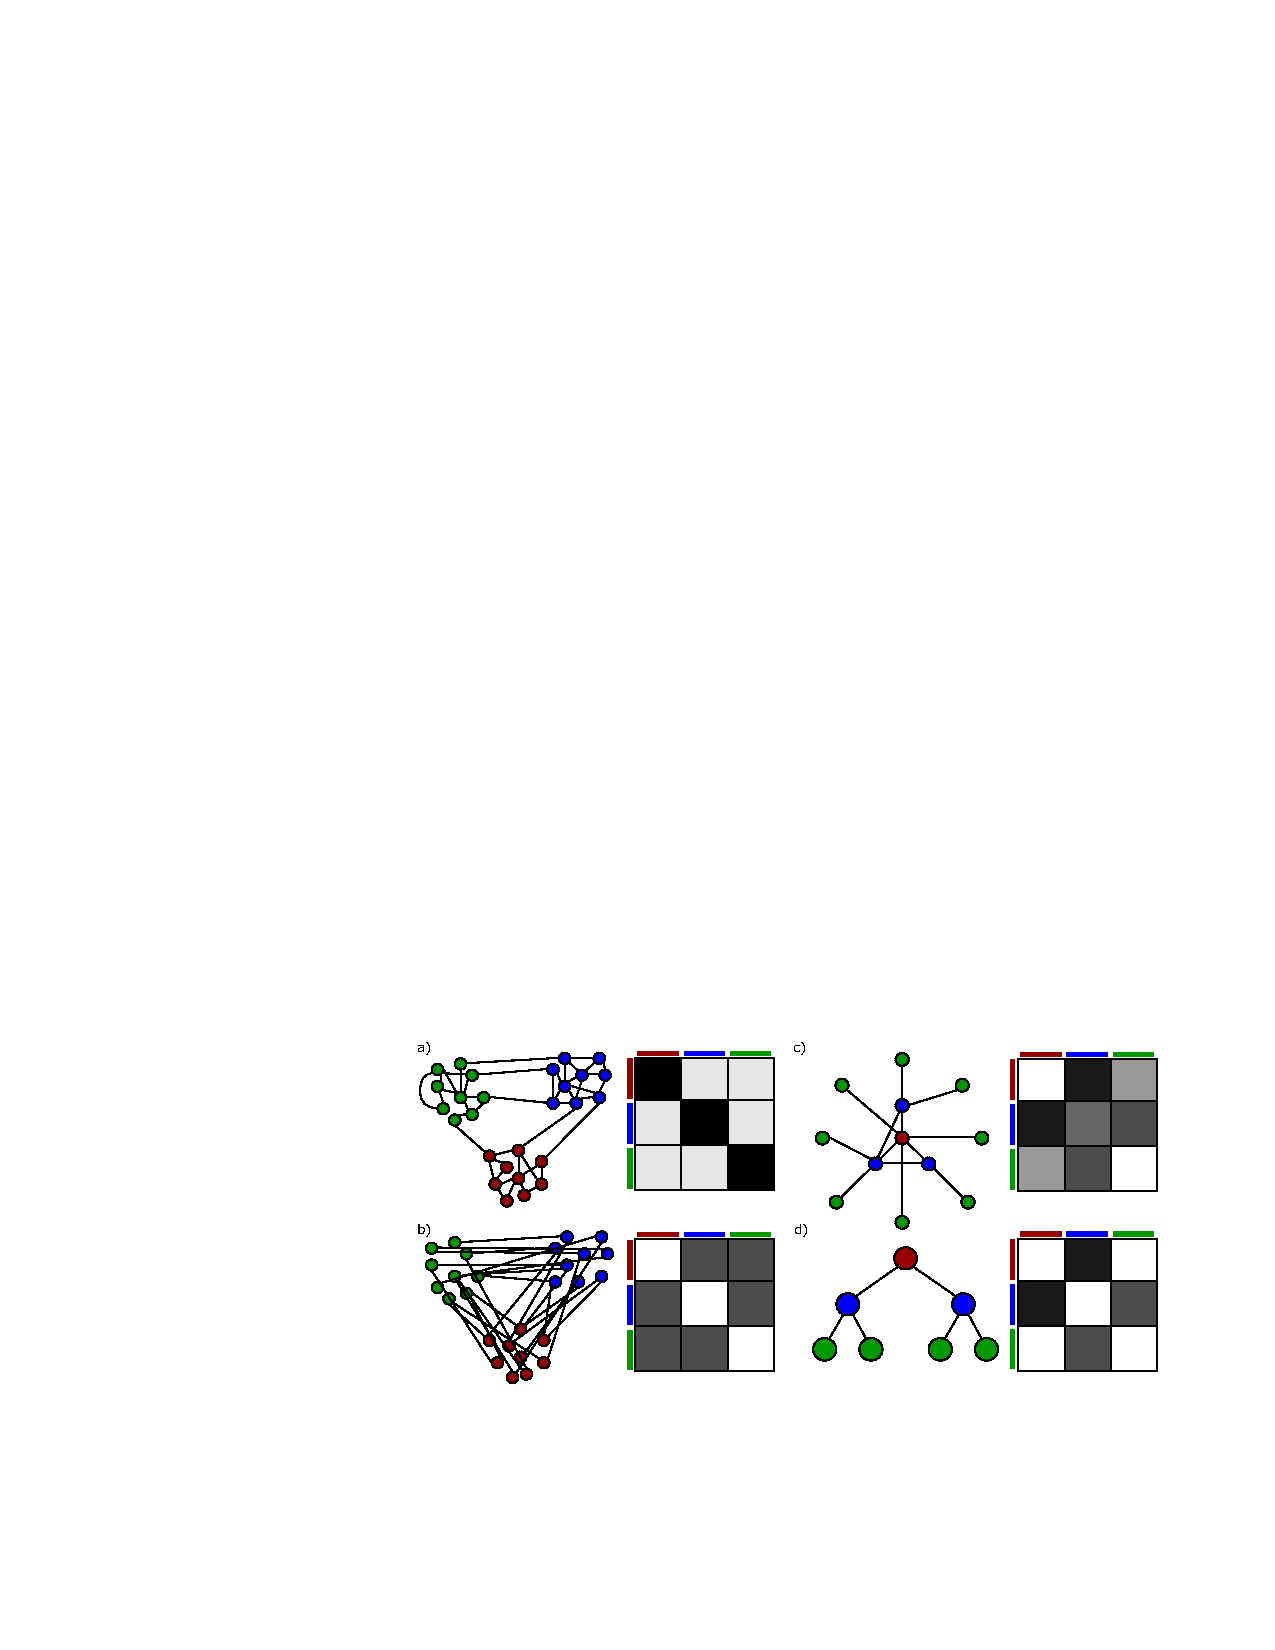
\includegraphics[width= 0.8\textwidth]{sbm}%
    \caption{Graphs and stochastic block models describing them. The darker the color, the higher the connection probability. This visualisation is taken from them from Funke \& Becker (2019).}
    \label{fig:adjacencymatricesgraphon}
\end{figure}
\noindent
The similarities of the graphon with the stochastic block model make the latter an ideal candidate to compare the benefits of the graphon model against and also to look for inspiration, given that the stochastic block model has been applied and researched for the past five decades.
    \section{Graphon}
The graphon was first defined as the limit of a sequence of dense graphs. 
This limit object is represented by a symmetric function called w, W, $\mathcal{W}$ or $\Theta$, hereafter referred to as $\Theta$. 
The function signature of the graphon function is $\Theta: [0,1]^2 \rightarrow [0,1]$. 
In words this tells us that $\Theta$ takes two real valued parameters between 0 and 1 and returns a real value between 0 and 1. 
A single graph can be sampled from the graphon, by sampling a value $x_i$ between 0 and 1 from a uniform distribution for each node $n_i$ and then adding edges between nodes $n_i$ and $n_j$ by drawing a sample from a Bernoulli distribution with probability $\Theta(x_i,x_j)=\Theta(x_j,x_i)$.
Since every node in the network is associated with a value $x_i$, this graphon approach is also termed a latent variable model.
This property makes it similar to the eigenmodel by \citeA{hoff2007}, which is also a latent variable model, albeit with a different definition of the latent space.
Due to the aforementioned sampling procedure, the function $\Theta$ can be seen as a continuous adjacency matrix and the graph defined by it is sometimes referred to as a W-graph \cite{latouche2016}. 
In figure \ref{fig:adjacencymatricesgraphon} this concept can be seen, where the graphon function appears to be a smooth version of the concrete adjacency matrix. 
\begin{figure}[H]
    \center
    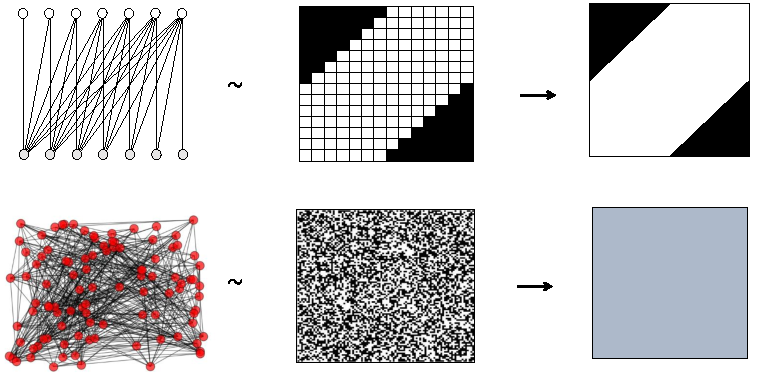
\includegraphics[width= 0.8\textwidth]{borgs2017graphon}%
    \caption{Graphs, adjacency matrices and graphons for the bipartite half graph (top) and a random graph (bottom). This visualisation is taken from Borgs \& Chayes (2017).}
    \label{fig:graphonexample}
\end{figure}
\noindent
To understand what the graphon as a limit object is representing, we have to understand what it is the limit of. 
This is however a field of active research, as multiple different answers can be given to this question. 
In this context we define convergence as follows: given a process that constructs graphs of arbitrary sizes with a certain property (e.g. bipartite), a sequence of graphs strictly increasing in size may converge with respect to a certain metric applied to the graphs.
In the example of a sequence made up of half graphs of increasing size, the convergence can be visualised as a smoothing of the adjacency matrix, as seen in figure \ref{fig:graphonexample}.
Convergence of graph sequences can be defined with respect to different metrics.
However, the first and still most prominent metric to define convergence by, is the cut metric, as defined by \citeA{lovasz2006}. 
The cut metric decreases to zero as the size of the graphs in a sequence continue to grow.
The following definition of the cut metric is taken from \citeA{memoli2016}:
Let G and G' be two graphs with node set $\{1, ..., n\}$. 
For Subsets S, T of $\{1, ..., n\}$, let $e_G(S,T)$ be the number of edges starting in S and ending in T (edges in the union S $\cup$ T counted twice.) Define their cut distance as
$$d_{cut}(G,G')=\underset{S,T \subseteq V(G)}{max}\dfrac{|e_G(S,T) - e_{G'}(S,T)|}{n^2}$$
The definition of the graphon as the limit of sequences of graphs has at least one important consequence related to the edge density it represents. 
Given that the graphon is defined for sequences of increasing size, the edge density of the graphs in the sequence tends to 0 if the amount of edges grows with $o(n^2)$.
Such a sequence is called a sequence of sparse graphs, while a sequence with a growth rate of $O(n^2)$ is called a sequence of dense graphs.
Thus, the graphon is zero almost everywhere for sequences of sparse graphs.
This might imply that graphon models (and all models they generalise) are misspecified for modelling real world graphs, which are often characterised as sparse, with related models producing sparse sequences \cite{wolfe2013}.\\\\
% A different definition of sparse and dense refers to the fraction of present edges out of all possible edges in a given graph.
% Here, a graph is said to be sparse if the amount of edges is very small compared to the amount of all possible edges.
% This definition is rather vague, but remains in use in the academic discourse surrounding network modelling.
% Therefore it's important to note that the sequence of dense graphs can consist entirely of sparse graphs, given that the amount of edges in the graphs of the sequence is small and grows with $O(n^2)$.
\noindent
There exists an older but related approach to modelling networks, which makes use of a slightly different formalism, called the representation theorem for exchangeable random graphs. 
This approach underlies nearly all random graph models, which have been thoroughly researched in the field of statistics \cite{hoover1979, aldous1981, kallenberg1990}. 
Work on showing that these two theories are two separate branches of network science that treat the same mathematical object, has been done by \citeA{diaconis2007} and \citeA{austin2008}. 
Both authors remarks show that the definition of the graphon as a graph limit allows for the application of algorithms and methods developed in the field of property testing to the graphon. \\\\
Furthermore, this work shows that graphon models generalise all random graph models that operate under the assumption of node exchangeability.
This includes models such as the Erd\H{o}s–Rényi random graph, the stochastic block model, the random dot product graph model and the infinite relational model \cite{Medina2020}.
The generalisations for the Erd\H{o}s–Rényi random graph and the stochastic block model have relatively short proofs that elucidate this concept of generalisation.
The random graph model can be written as $G(N,p)$ where $N$ is the amount of nodes in the graph and $p$ is the probability that an edge between two nodes exists. 
Thus to draw a sample from the graph defined by $G(N,p)$, we have to sample for every edge $(n_i, n_j)$ from the Bernoulli distribution $\text{Bern}(p)$, the outcome of which determines the presence of edge $(n_i, n_j)$. 
An equivalent definition making use of the graphon model can be achieved as follows: For $N$ nodes, sample for each node $n_i$ a value $x_i$ as $x_i\sim \text{Uniform}(0,1)$ and sample edges between nodes $n_i$ and $n_j$ by sampling from $\text{Bern}(\Theta(x_i, x_j))$ where $\Theta$ is defined as $\forall x_i,x_j \in [0,1]: \Theta(x_i, x_j)=p$. If $N$ and $p$ are equal to the values chosen in the random graph model, this graphon model describes the same distribution over graphs as the random graph model.\\
Analogously, the stochastic block model can also be defined in terms of a graphon model. 
The standard definition of the stochastic block model is given as follows: 
For a model with $k$ blocks, sample for every node $n$ its block membership $x$ from a discrete uniform distribution $x \sim \text{Uniform}(1,k)$.
Now sample for every edge $e_{ij} = (n_i, n_j)$ from the Bernoulli distribution $e_{ij} \sim \text{Bern}(P_{ij})$, where $P_{ij}$ is the probability, that an edge between nodes in block $i$ and $j$ exist.
The equivalent graphon definition can then be given by the following: 
For $N$ nodes, sample for each node $n$ a value $x$ as $x\sim \text{Uniform}(0,1)$ and sample edges between nodes $n_i$ and $n_j$ by sampling from $\text{Bern}(\Theta(x_g, x_h))$ where $\Theta$ is defined as a piece wise constant function, made up of $k^2$ pieces of equal size. The value of $\Theta$ is then determined by $\forall x_g \in [(i-1)*\dfrac{1}{k},i*\dfrac{1}{k}]: \forall x_h \in [(j-1)*\dfrac{1}{k},j*\dfrac{1}{k}]: \Theta(x_i, x_j)=P_{ij}$. When $P_{ij}$ is the probability distribution mentioned in the stochastic block model, this graphon model becomes equivalent to the stochastic block model. The stochastic block model as a special case of the graphon model can be used to approximate the graphon \cite{airoldi2013,latouche2016,pensky2019,peng2022}. This further shows the strong connection of these two models. 
This strong connection between the graphon model and the stochastic block model, which has already been successfully used in connectomics, indicates that the graphon model might similarly be useful to model networks in connectomics.

% Furthermore, it allows us to , it raises questions about how the limits of graphons apply to stochastic block models. Whereas the definition of graphons leads to dense graphs, stochastic block models do not have the same theoretical background and have thus readily been modified to take sparsity into account explicitly \cite{gyenge2010, noroozi2021}.\\\\

% These advantages seemingly make graphon models interesting to the field of connectomics, as we have previously used random graph models to great success.
    \section{Gaussian Processes}
In the field of statistical modelling, there has been a continuous effort to model functions in a systematic, theory-driven way. On the one hand, statistical models should be as simple as possible, such that they remain tractable for quick calculations. On the other hand, they should also allow for enough complexity to grasp the intricacies of the phenomenon underlying the data. For this reason, Bayesian nonparametric models have seen rising interest, as they combine multiple nice properties. Their model complexity expressed by the amount of parameters in the model grows with the available data, while giving guarantees on over and under fitting to the data. One of the most prominent approaches in Bayesian nonparametric modelling is the Gaussian process model. As with all Bayesian models, we are interested in learning the posterior distribution given the likelihood and the prior distribution like this:
\begin{align}
\label{basicbayes}
\text{posterior} = \dfrac{\text{likelihood} * \text{prior}}{\text{marginal likelihood}}
\end{align}

In the context of the graphon model, the posterior is comprised of the joint distribution over the function $\Theta$ and the latent variables $U$ forming the input to $\Theta$. The likelihood is the probability of the data $X$ given a model and the prior describes the prior probability on the function $\Theta$ and the latent variables $U$. Thus formula \ref{basicbayes} becomes:
\begin{align}
\label{bayes2}
p(\Theta, U\mid X) = \dfrac{p(X|\Theta,U) * p(\Theta,U)}{p(X)}
\end{align}
To understand the Gaussian process model approach, one needs to take a close look at a few different components of the model. The most interesting parts are the Gaussian process prior and its hyperparameters.
    \subsection{Gaussian Process Prior}
The most succinct definition of a Gaussian process prior is that it's a \say{collection of random variables, any finite number of which have a joint Gaussian distribution} \cite[~p. 13]{rasmussen2005}. The joint distribution is defined by the mean function $m(x)$ and the covariance matrix $k(x,x)$, where $k$ is a kernel function (also called covariance function) that returns a covariance matrix and $x$ refers to the set of points at which we evaluate the Gaussian process. Following this definition, it is possible to use Gaussian processes to put a prior on functions, by choosing appropriate mean and kernel functions. In many applications, a mean of zero can be assumed, which simplifies the calculations that need to be made. Furthermore, the squared exponential kernel (also called Gaussian kernel or radial basis function kernel) is commonly used as the kernel function. This is because it encourages smooth functions and has few parameters, namely the length scale $\ell$ and the signal variance $\sigma^2$, which is sometimes referred to as output variance or scale factor. This kernel function can be written like this:
$$ k(\sigma^2,\ell;x,x')=\sigma^2\exp{\left( -\dfrac{(x-x')^2}{2\ell^2} \right) } $$
The parameters $\sigma^2$ and $\ell$ are usually omitted from the function signature, like so:
$$ k(x,x')=\sigma^2\exp{\left( -\dfrac{(x-x')^2}{2\ell^2}\right)} $$
\subsection{Hyperparameters}
The parameters $\sigma^2$ and $\ell$ of the function $k$ are also called hyperparameters, as they define the function which defines the parameters of the prior for $\Theta$. 
\subsection{Inference in Gaussian Process Models}
In the context of Bayesian models, of which Gaussian processes are a specific case, inference is the process of updating the prior distribution with data to arrive at the posterior distribution.\\\\
In Gaussian processes, the prior also includes hyperparameters, which are thus an important part in model inference. 
These hyperparameters can either be optimised for, resulting in a point estimate of them, or they can be integrated out numerically using MCMC techniques. 
\subsubsection{Optimising}
Optimising the hyperparameters is usually done by choosing the hyperparameters that maximise the marginal likelihood, as this procedure minimises over and under fitting to the data. Furthermore, using the marginal likelihood as a loss function allows for the usage of gradient descent to optimise the hyperparameters. Since this method yields a single set of hyperparameters, there is no guarantee on whether the results are a global or a local maximum. However, optimisation requires computational resources compared to MCMC methods.
\subsubsection{MCMC}
MCMC methods can sample from the posterior distribution directly, which means that instead of optimising point estimates of the hyperparameters, the full joint posterior distribution, including hyperparameters is estimated \cite{candela2005, nickisch2008}.
The main drawback to MCMC based methods is however that many samples need to be drawn, which is usually a compute intensive task. 
Furthermore, the samples drawn from the posterior distribution via MCMC are only guaranteed to converge to the true posterior after an infinite amount of samples are drawn.
Stopping the MCMC chain early thus needs to be justified by showing convergence of the samples drawn from the chain.\\\\
In the context of graphs, the data consists of binary information relating to the existence of edges for a given node pair. This means that the likelihood does not have a Gaussian form, which together with the Gaussian prior implies that there is no closed form solution for the marginal likelihood. This in turn makes the use of approximation techniques such as MCMC mandatory.
\section{Random Function Model}
\citeA{lloyd2012} have created the Random Function Model (RFM), a Bayesian nonparametric model that estimates the graphon for a given graph. This approach is highly promising as it makes use of the advantages of fully Bayesian Gaussian processes and closely follows the mathematical definition of the graphon.

\subsection{Model Definition}
As a Bayesian model, the RFM performs inference on the posterior distribution using Bayes rule as defined in \ref{bayes2}. The RFM estimates the graphon function $\Theta$ from a dataset of a graph, using a Gaussian process prior. 
\subsubsection{Prior}
The prior of the RFM consists of a set of latent variables $U$, hyperparameters $\Phi={\ell,\sigma,s}$ and kernel function $k(x,x')$. As mentioned earlier, in a graphon model, every node of a network has a latent variable assigned. In this case, the set $U$ consists of all latent variables for the nodes in a graph of size $n$. 
Thus, U is sampled as $U = {U_1,U_2,...,U_n} \sim \text{Uniform}(0,1)$. The three hyperparameters that define the exact kernel function are sampled from log normal distributions as follows:
$\ell \sim \text{Lognormal}(1,0.5) $, $ \sigma \sim \text{Lognormal}(0.1,0.5) $ and $s \sim \text{Lognormal}(2,0.5)$. $\Psi$ refers to the complete set of hyperparameters like this: $\Psi=\{\ell,\sigma,s\}$. Finally the kernel function is defined building upon the well known squared exponential kernel, applying it once on the input and again on the mirrored input, to enforce symmetry. As the graphon function is defined on edges (pairs of nodes), the kernel function of the rfm model is defined on pairs of edges, as it determines the strength of the influence that a single point (an edge) in the graphon function has on another point (another edge). Following the authors of the RFM, a single edge is defined as $\xi_{i,j}=\xi_{U_i,U_j}=(U_i, U_j)$, whereas the set of all edges is defined as $\xi = \{\xi_{i,j}|\forall i, j \in U \}$. A flipped edge is noted using a bar above, thus if $\xi_{i,j}=(U_i, U_j)$ then $\bar{\xi}_{i,j}=(U_j, U_i)$. The kernel function is then given by 
$$
sek_\Psi(\xi_{ij}, \xi_{gh}) = s^2\exp(\dfrac{-|\xi_{ij}-\xi_{gh}|^2}{2\ell^2}) $$
$$\bar{k}_\Psi(\xi_{ij}, \xi_{gh}) = \dfrac{1}{2}(sek_\Psi(\xi_{ij}, \xi_{gh}) + sek_\Psi(\xi_{ij}, \bar{\xi}_{gh}))$$
$$k_\Psi(\xi, \xi') = (\forall \xi_{ij} \in \xi: \forall \xi_{gh} \in \xi': \bar{k}_\Psi(\xi_{ij}, \xi_{gh}) )+ \sigma^2I $$

In the above formulas, $sek_\Psi(\xi_{ij}, \xi_{gh})$ is the squared exponential kernel, whereas $\bar{k}_\Psi(\xi_{ij}, \xi_{gh})$ applies $sek_\Psi$ on the input and the mirrored input, finally $k_\Psi(\xi, \xi')$ is a function that takes sets of edges as parameters and applies $\bar{k}_\Psi$ to all possible pairs of edges. This last definition of the kernel function results in a matrix of the following form: 
        $$
	\begin{bmatrix} 
	k_\Psi(\xi_1, \xi_1) +\sigma^2 & \cdots & k_\Psi(\xi_1, \xi_n) \\
	\vdots &  \ddots & \vdots \\
	k_\Psi(\xi_n, \xi_1) & \cdots & k_\Psi(\xi_n, \xi_n) +\sigma^2 \\
	\end{bmatrix}
	\quad
	$$

The previously mentioned components of the prior are subsumed in the notation: $$\Theta \sim \text{GP}(0,k_{\Phi})$$
\subsubsection{Likelihood}
The observed graph data $X$ comes in the form of the symmetric binary adjacency matrix of a graph of rank $n$, where $n$ is the amount of nodes in the graph. Thus the observed edge between node $n_i$ and $n_j$ is defined to be $X_{ij} = X_{ji}$. Note that $X$ denotes observed graphs, whereas $\xi$ denotes samples from the RFM. Given that the data is binary, as it represents the presence of an edge in a graph, the probability of a single edge existing is defined by a Bernoulli distribution. Furthermore, the RFM approximates the graphon function as unbounded, which implies that the estimate of the graphon function can't directly be used as a probability. To circumvent this issue, a link function $\phi(w)$ is used that transforms the unbounded values of the graphon function to the space of real numbers between 0 and 1. The specific link function in the RFM is the logistic function, which is defined as $\phi(w) = \dfrac{1}{1+\exp{(-w)}}$. 
Thus the probability of a certain edge $X_{i,j}$ in the observed graph existing according to the RFM is $p(X_{i,j}\mid \Theta, U, \Psi) = \text{Bern}(\phi(\Theta(U_i, U_j)))$. The complete model likelihood is the product of the probability of all single observations given the model, thus it can be written as $p(X\mid\Theta,\Psi,U) = \prod_{i=0}^n \prod_{j=0}^n p(X_{i,j}\mid\Theta,U))$.
\subsection{Full Model}
The full Bayesian theorem of the model can now be written as follows:
\begin{align}
\label{fullmodelbayes}
p(\Theta,\Psi,U\mid X)=\dfrac{p(X\mid\Theta,\Psi,U)p(\Theta,\Psi, U)}{p(X)}
\end{align}
The full definition of the model prior is then given by the following:
\begin{align}
\ell &\sim \text{Lognormal}(1,0.5)\\
\sigma &\sim \text{Lognormal}(0.1,0.5)\\
s &\sim \text{Lognormal}(2,0.5)\\
\Psi &= \{\ell, \sigma, s\}\\
U = {U_1,U_2,...,U_n} &\sim \text{Uniform}(0,1)\\
\xi_{i,j}=\xi_{U_i,U_j}&=(U_i, U_j)\\
\xi &= \{\xi_{i,j}|\forall i, j \in U \}\\
sek_\Psi(\xi_{ij}, \xi_{gh}) &= s^2\exp(\dfrac{-|\xi_{ij}-\xi_{gh}|^2}{2\ell^2})\\
\bar{k}_\Psi(\xi_{ij}, \xi_{gh}) &= \dfrac{1}{2}(sek_\Psi(\xi_{ij}, \xi_{gh}) + sek_\Psi(\xi_{ij}, \bar{\xi}_{gh}))\\
k_\Psi(\xi, \xi') &= (\forall \xi_{ij} \in \xi: \forall \xi_{gh} \in \xi': \bar{k}_\Psi(\xi_{ij}, \xi_{gh}) )+ \sigma^2I \\
\Theta &\sim \text{GP}(0,k_\Psi)
\end{align}
The full likelihood definition is given by:
\begin{align}
\Theta(U_i, U_j) &= \Theta(\xi_{i,j})\\
\label{single_edge_llh} p(X_{i,j}|\Theta(U_i, U_j)) &= \text{Bernoulli}(\phi (\Theta(U_i, U_j)))\\
\label{complete_llh}
p(X|\Theta) &=  \prod_{i=0}^n \prod_{j=0}^n p(X_{i,j}|\Theta(U_i, U_j))
\end{align}

% However, the RFM model samples from a standard normal distribution instead of a uniform distribution over the range $(0,1)$. The authors defend this deviation from the standard definition of the graphon by mentioning that sampling from a normal distribution is more convenient during inference, while this definition is equally valid as the definition of $\Theta$ on the unit square. 
\subsubsection{Approximations}
A few changes to the above model help to make it more tractable and easier to implement on current hardware.\\\\
First, $U$ is sampled from a normal distribution, which changes the parameters of $\Theta$ from real numbers between 0 and 1 to $\mathbb{R}^2$. This needs to be taken into account when sampling from the model, but has no further implications on the underlying graphon theory.\\\\
Second, since the complexity of the Gaussian process calculations is cubic in the size of the set of observed edges, the authors made use of the subset of regressors approximation technique \cite{candela2007}. In this technique, we approximate the evaluation of $\Theta$ by introducing a set of pseudo points $\eta$ of size $m$ that summarise the data. \\\\
The above approximations only influence the model prior, which is now defined as follows:
\begin{align}
\ell &\sim \text{Lognormal}(1,0.5)\\
\sigma &\sim \text{Lognormal}(0.1,0.5)\\
\text{s} &\sim \text{Lognormal}(2,0.5)\\
\Psi &= \{\ell, \sigma,\text{s}\}\\
U = U_1,U_2,...,U_n &\sim \mathcal{N}(0,I_n)\\
\xi_{i,j}&=(U_i, U_j)\\
\xi &= \{\forall i, j \in U: \xi_{i,j}\}\\
\eta = \eta_1,\eta_2,...,\eta_m &\sim \mathcal{N}(0,I_m)\\
\bar{k}_\Psi(\xi_1, \xi_2) &= s^2\exp(\dfrac{-|\xi_1-\xi_2|^2}{2\ell^2})\\
k_\Psi(\xi_1, \xi_2) &= \dfrac{1}{2}(\bar{k}_\Psi(\xi_1, \xi_2) + \bar{k}_\Psi(\xi_1, \bar{\xi_2})) + \sigma^2I\\
T &\sim \mathcal{N}(0,k_\Psi(\eta,\eta))\\
\Theta &= k_\Psi(\xi,\eta) k_\Psi(\eta,\eta)^{-1}T
\end{align}
Adding the additional parameters to the Bayesian theorem in equation \ref{fullmodelbayes} yields equation \ref{approxmodelbayes}.
\begin{align}
\label{approxmodelbayes}
p(\Theta,\Psi,T,U,\eta\mid X)=\dfrac{p(X\mid\Theta,\Psi,T,U,\eta)p(\Theta,\Psi, T, U, \eta)}{p(X)}
\end{align}

\subsection{Implementation}
Given that we try to infer the posterior distribution $\text{P}(\Theta,\Psi,T,U,\eta\mid X)$, we would need to calculate the likelihood, the prior and the marginal probability. 
However, since the likelihood is not Gaussian, we cannot calculate the posterior analytically, as we would have to integrate over all possible prior values, which is intractable. 
To circumvent this, a Markov Chain Monte Carlo approach is used to directly sample from the posterior distribution.
This is done using elliptical slice sampling \cite{murray2010} for the random variable $T$, while slice sampling \cite{neal2003} is used for all other random variables. 
The original MATLAB implementation \footnote{\url{https://jamesrobertlloyd.com/assets/BasicRFM.tar.gz}} is still available. 
A reimplementation\footnote{\url{https://github.com/adiehl96/master/tree/main/pyrfm}} in Python was created for this work, which is available as well.
%-------------------------------------------------------------------------------------------------------------------------------------------------------------------------------------------------------------------
% \chapter{Preliminaries}\label{preliminaries}
% -------------------------------------------------------------------------------------------------------------------------------------------------------------------------------------------------------------------
\chapter{Methods}
To investigate the guiding research question a number of experiments are presented in this chapter. 
\section{Data}
The RFM is being investigated using two dataset originating from brain scans of healthy young adults.
\subsection{Human Connectome Project}
The human connectome project (HCP).
This dataset consists of 100 diffusion MRI measurements of 100 unrelated subjects between the ages of 25 and 35 \cite{vanessen2012}.
The data was preprocessed using the method described by \citeA{Amico2018}, resulting in structural connectivity graphs of rank 164, using Destrieux parcellation \cite{destrieux2010}.
This data was further processed from weighted matrices to binary matrices using consistency thresholding \cite{roberts2017}. The final result of these preprocessing steps are simple, symmetric, binary graphs, with an edge density of approximately 20\%.
\subsection{MICA-MICs}
\citeA{royer2021} provide a dataset of diffusion MRI data for 50 healthy young adults. Next to the raw measurements, this dataset also contains processed structural connectivity graphs for different parcellations. These connectivity graphs are further processed, similar to how the HCP is processed, using consistency thresholding to derive a simple, symmetric, binary graphs with a density of 20\%. The graph property values before and after thresholding
\begin{table}[h]
\caption{Graph properties for the MICA-MICs dataset and for the MICA-MICs dataset after consistency thresholding.}
\begin{tabular}{|l|l|l|l|}
\hline
 & \textbf{MICA-MICs} & \textbf{Consistency Thresholded MICA-MICs}  \\ \hline
Density           & 0.970 $\pm$ 0.017  & 0.200 $\pm$ 0.000 \\ \hline
Transitivity      & 0.989 $\pm$ 0.013  & 0.019 $\pm$ 0.015 \\ \hline
Local Efficiency  &  N.a. $\pm$ N.a.   & 0.756 $\pm$ 0.000 \\ \hline
Global Efficiency & 0.959 $\pm$ 0.009  & 0.556 $\pm$ 0.000\\ \hline
Degree Assortativity Coefficient  & -0.025 $\pm$ 0.007 & -0.039 $\pm$ 0.001 \\ \hline
Average Clustering Coefficient    & 0.972 $\pm$ 0.012  &  0.541 $\pm$ 0.001 \\ \hline
\end{tabular}
\end{table}
As is evidenced by the low standard deviations, the networks are highly homogeneous.
\section{Experiments}
In order to test the usefulness of the graphon estimation approach to connectomics, several experiments were conducted. In addition to the experiments described here, convergence and ablation tests can be found in the appendix.
\subsection{Graphon Recovery} \label{provengraphonexperiment}
According to the research question, the modelling ability of the RFM is investigated. 
Modelling here refers to the estimation of the graphon function for a given graph. 
Since the graphon of brain networks is not known a priori, in this first experiment, a graph sampled from a predefined graphon will be used to train the RFM.
For this experiment, three types of graphon functions will be used, namely a bipartite graphon, a scale free graphon and a community graphon.
A bipartite graphon produces graphs that consist of two groups of nodes, which have no connections within their group, while being fully connected to the nodes in the other group.
The scale free graphon refers to a graphon that produces graphs in which the degree frequency diminishes exponentially as the degree grows. The exact formula for this graphon was taken from \citeA{latouche2016}.
Finally, the community graphon is a graphon which produces graphs that exhibits highly connected clusters of nodes connected by relatively few nodes.
All three of these graphon functions are visualised in the figures \ref{estimatedbipartitegraphon}, \ref{estimatedscalefreegraphon} and \ref{estimatedcommunitygraphon} respectively.
The estimated graphon is first visually compared to the predefined graphon, and subsequently graphs are sampled from the estimated and the predefined graphon and compared using several graph metrics.
The graph metrics that are used are chosen for their relevance in connectomics, as well as for their sensitivity to the three predefined graphons used in this experiment.
The exact graph properties used are the following:
\begin{enumerate}
    \item Graph Density \shortcite{rubinov2010,farahani2019}
    \item Transitivity \shortcite{rubinov2010, ingalhalikar2014}
    \item Local Efficiency \cite{rubinov2010, betzel2022}
    \item Global Efficiency \cite{rubinov2010, betzel2022}
    \item Degree Assortativity Coefficient \shortcite{rubinov2010, lim2019}
    \item Average Clustering Coefficient\shortcite{rubinov2010, vecchio2017}
\end{enumerate}
This experiment shows, how closely the estimated graphon functions resemble the actual graphons that produced the graphs.
\subsection{Single Subject Link Prediction Comparison} \label{singlelinkpredictionexperiment}
In this experiment, the graph of an individual subject will be partitioned into a training set and a test set. 
After training on the training set, the method will predict the test set. 
The prediction and the ground truth will be used to calculate the area under the curve of the receiver operator characteristic (AUROC). 
A comparison is made with widely used but closely related models. That is on the one hand the Eigenmodel by \citeA{hoff2007} and on the other missSBM by \citeA{barbillon2022}. 
These models are both latent variable random graph models which are generalised by the random dot graph \cite{matias2014} which in turn is generalised by the graphon \cite{Medina2020}. 
Thus, this experiment shows whether the link prediction performance is greater than in models generalised by the graphon, which directly answers the main research question of this thesis, at least in relation to link prediction. 
% \subsection{Group Link Prediction Comparison}
% In the RFM it is possible to learn from multiple connectomes before predicting a certain hold out test set. 
% In two simple symmetric binary graphs created from brain imaging data that have been processed using the same brain parcellation, edges represent connections between the same regions of interest in the brain. 
% Furthermore, since the connections in the connectomes of healthy young adults are largely similar, the precise connectome that one individual has, should be informative for the connectome that another individual has. 
% Therefore, if the RFM is being trained on full connectomes of some individuals and 80\% of the connectome of individual $i$, then the link prediction on the held back 20\% should be improved compared to the link prediction done by only training on the 80\% of individual $i$.
% This experiment directly relates to hypothesis 3, which suggests that the graphons estimated for structural connectivity networks of healthy young adults are similar.
% If these graphons are indeed highly similar, then this experiment should show an increase in predictive ability.
\subsection{Connectome Sample Quality}
\label{samplequalityexperiment}
Connectomics has long used graph properties to show statistical deviation from the brains of healthy adults. As mentioned previously, transitivity is one such graph property that has been found to correlate with creativity, but also with disorder severity for disorders of consciousness. Using graph properties such as transitivity are thus known to be relevant for the structure of the human structural connectome. 
It is therefore important that network models in connectomics are sensitive to these graph properties in order to model biologically plausible graphs. 
To test whether the RFM is sensitive to graph properties that are important to connectomics, a number of such properties will be computed for the MICA-MICs dataset and subsequently computed again for graphs sampled from the RFM.
If the RFM is well suited to model connectomics data, the expectation is that the graph properties will be similar between the MICA-MICs dataset and the sampled graphs.
This experiment is directly linked to assessing the main research question in so far as the RFM model captures the graph structure of the human connectome. The same graph properties are used as during experiment \ref{provengraphonexperiment}
\subsection{Graphon Based Graph Comparison}
As mentioned earlier, connectomics makes use of graph measures, such as transitivity. 
However, a recurring problem with using graph measures to compare graphs in the connectomics domain is that most graph measures are sensitive to the size of the network \cite{vanwijk2010}. 
In combination with the fact that the graph size of connectivity matrices in connectomics depends on the parcellation choice, this sensitivity to graph size limits the applicability most graph measures.
The graphon offers a potential solution to this problem, as it produces graphs with the same properties at any scale.
Given two graphs, $G1$ and $G2$ that represent the same network at different scales respectively at size $n$ and size $m$ with $n<<m$.
Let $GE1$ and $GE2$ be the graphon estimates of $G1$ and $G2$ respectively.
Assume that the graphon estimates model their observed graph well in terms of relevant graph properties.
Then the graph properties for graphs sampled from graphon estimate $GE1$ at size $l$ should be close to the graph properties for graphs sampled from $GE2$ at size $l$.
If the difference indicated by the graph properties for the sampled graphs is smaller compared to the difference indicated by the graph properties of the observed graphs, then using the graphon as an intermediate step solves the issue of comparing graphs of differing sizes.
For this experiment, MICA-MICs datasets will be used, as the authors provide parcellated structural connectivity data with different amounts of regions of interest for the same individual.
It is therefore given that the connectivity networks describe the underlying structure at different resolutions, making it ideal for this experiment.
For this experiment, two simple symmetric binary graphs of different sizes per subject will be used to learn a graphon.
The parcellation selected is that defined by \citeA{vosdewael2020}, as it is available at a size of 100 and 200.
Both graphons will be used to sample graphs of size 150, as this graph size is equidistant from either graph size.
The graph measures mentioned in experiment \ref{samplequalityexperiment} will be applied to the observed graphs and to the sampled graphs.
The mean and standard deviation of these graph properties for sampled graphs from both graphons as well as the graph properties from the observed graphs will subsequently be compared.
Finally the distance of these quantities will be computed. 
If this distance is smaller for the sampled graphs compared to the observed graphs, the graphon is a useful tool comparing graphs of different sizes.
This experiment concerns the second hypothesis as written in section \ref{researchquestion}, as it addresses the question of whether the graphon can help to compare graphs of different sizes.
\subsection{Visualisation}
The visualisation of the graphon function reveals certain patterns at a glance according to \citeA{lloyd2012}. The authors mention that stochastic equivalence is visible as block structure in the adjacency matrix, when the nodes are sorted according to their latent positions $U$ as estimated by the RFM. Furthermore, the authors mention that concentration of edges along the diagonal indicates homophily, which represents the affinity of nodes to connect to similar nodes, where similarity refers to a short distance between nodes in the latent space of the graphon.
These concepts can usually not be expressed in a single number, as these are not well defined concepts in network science.
Nevertheless, visualisation of the graphon function and the ordered adjacency matrix might still be valuable, if it can reveal certain graph properties at a glance.
If the graphon estimated by the RFM is stable after successive estimation procedures, this would point to a unique ordering of the nodes for every graph, something that is not usually available for networks.
% -------------------------------------------------------------------------------------------------------------------------------------------------------------------------------------------------------------------
\chapter{Results}
\section{Graphon Recovery}
\label{provengraphonresult}
\subsection{Bipartite Graph}
\begin{figure}[H]
    \center
    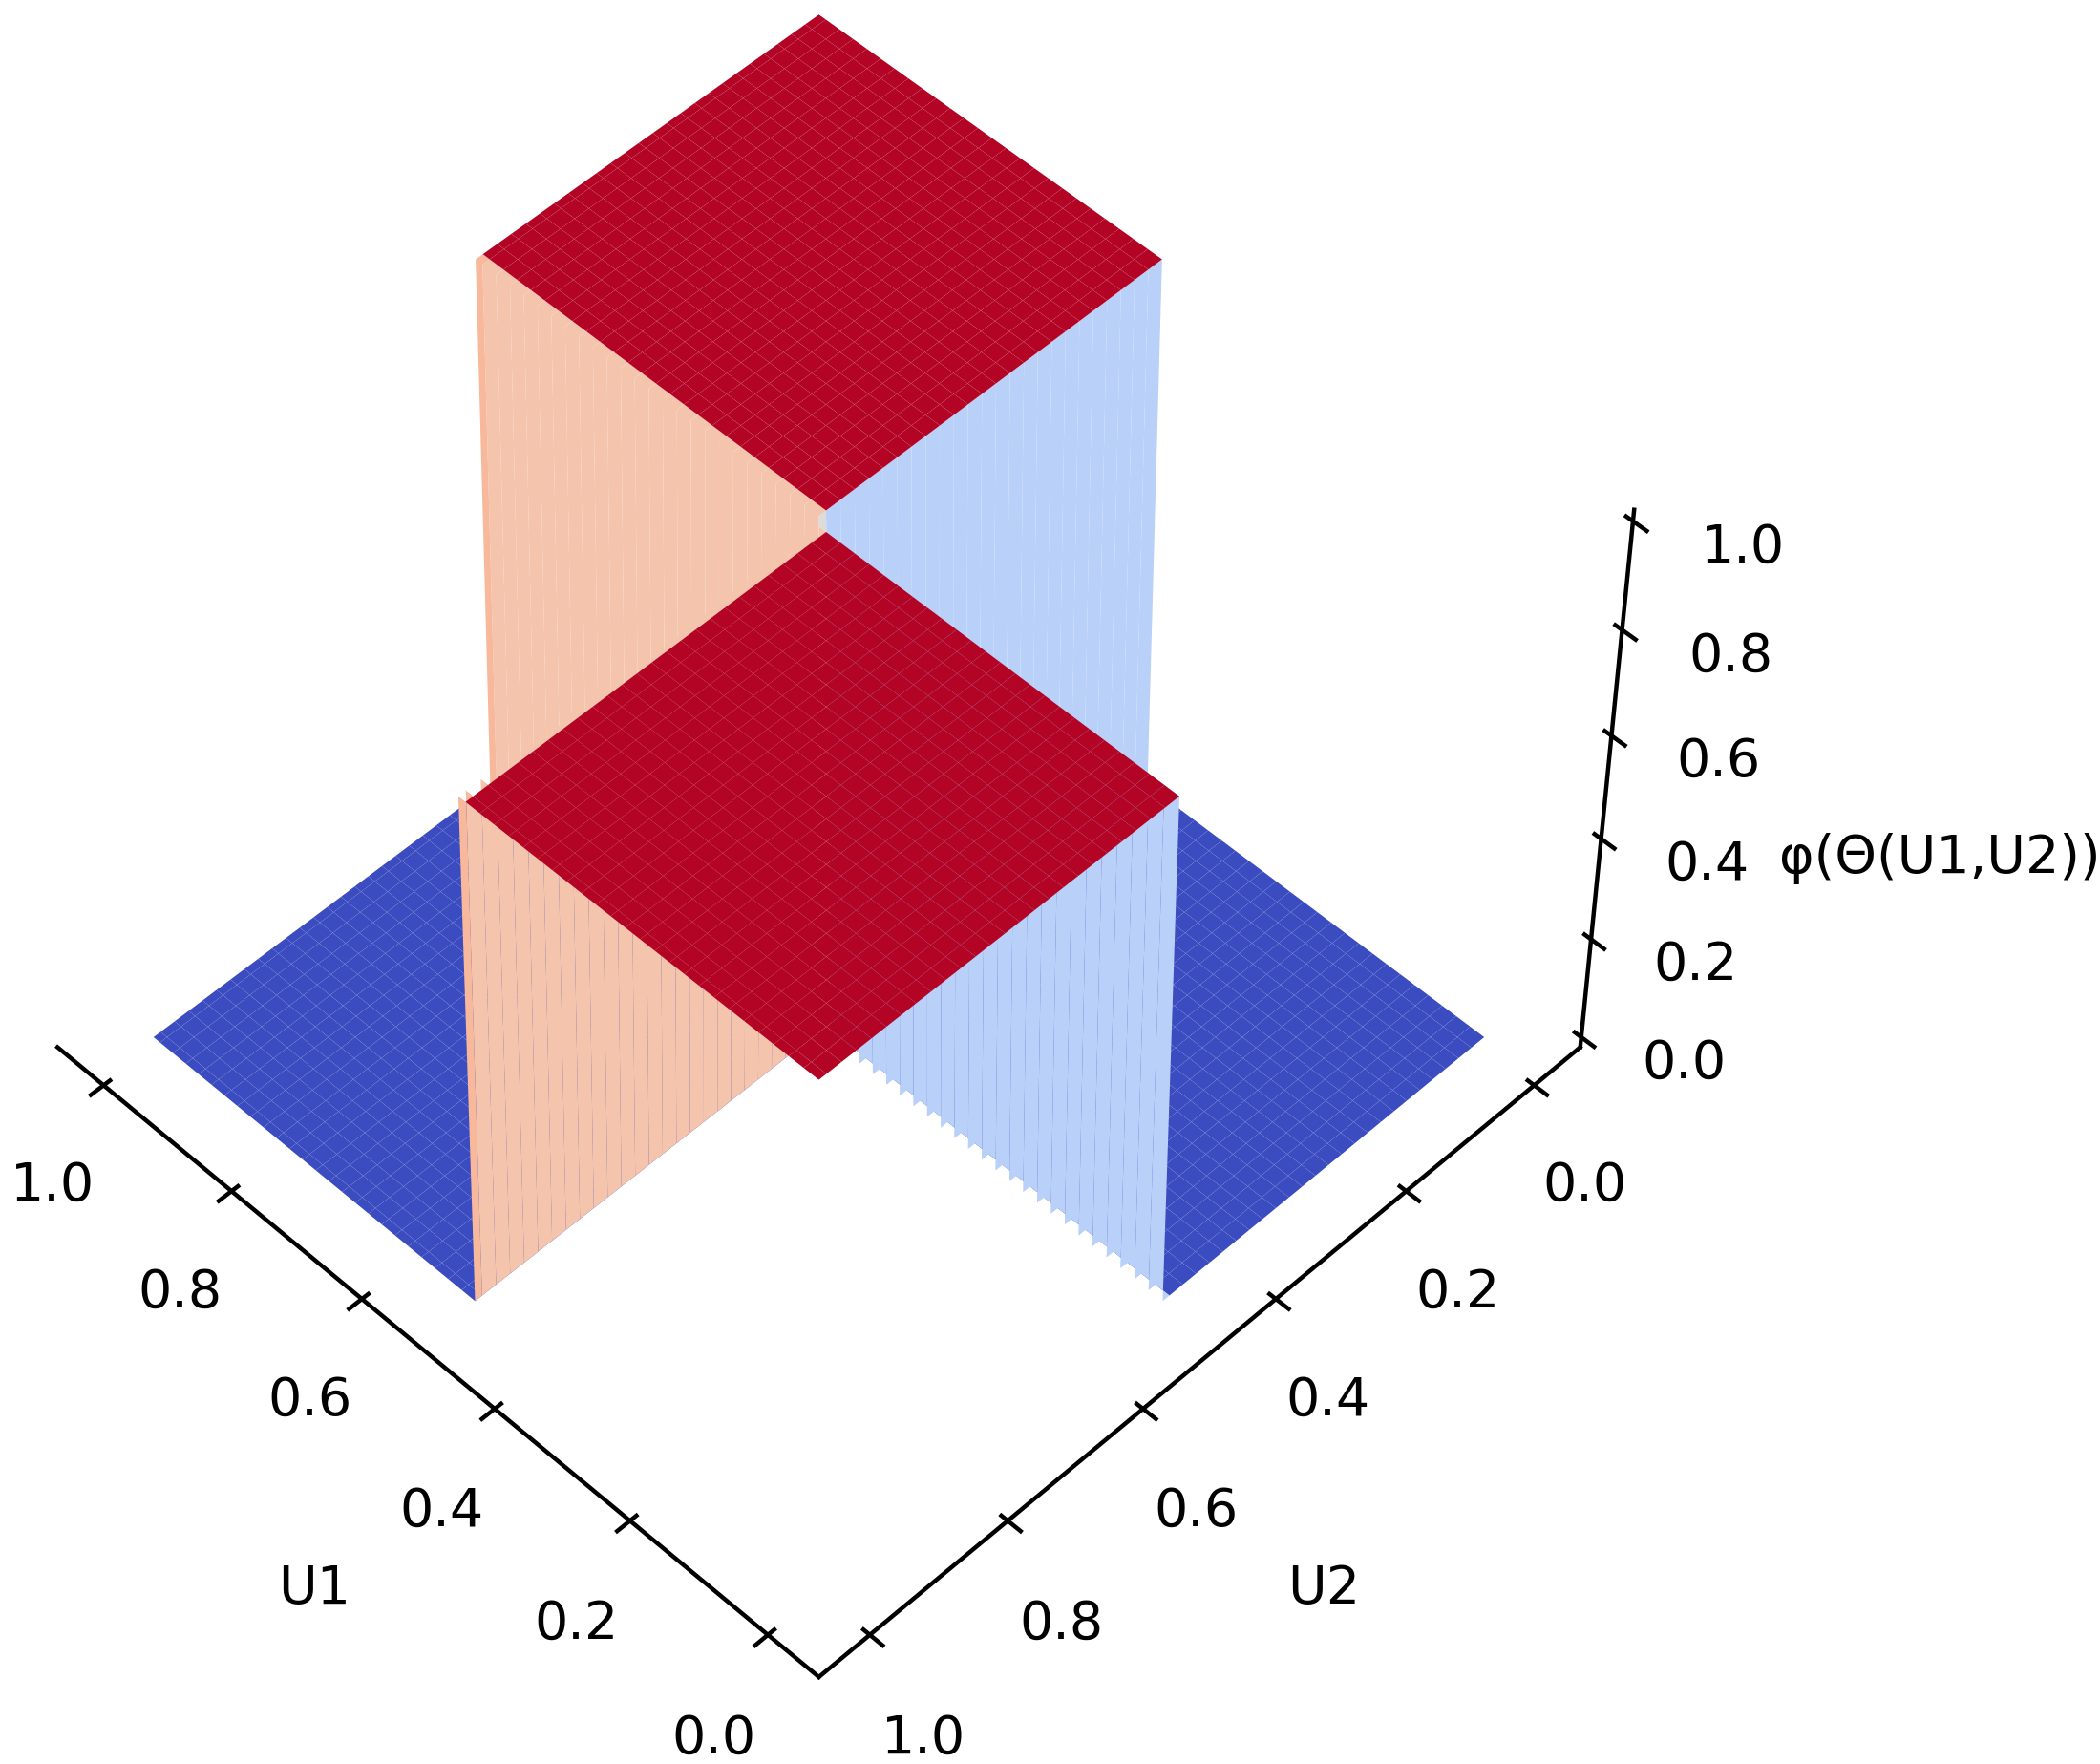
\includegraphics[width= 0.35\textwidth]{bipartitegraphon}%
    \hfill
    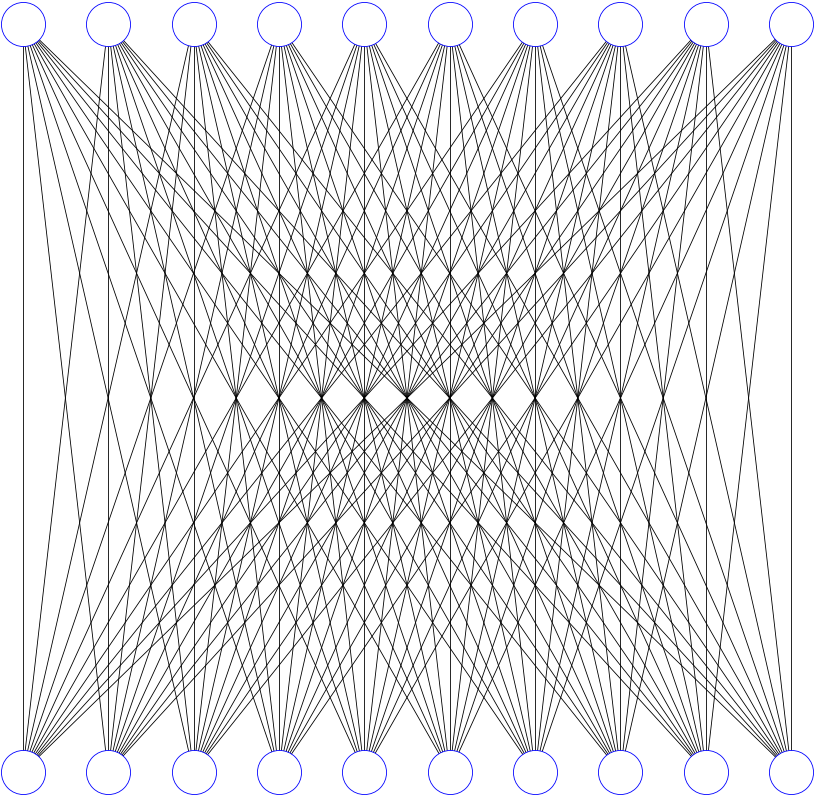
\includegraphics[width= 0.25\textwidth]{bipartitegraph}%
    \hfill
    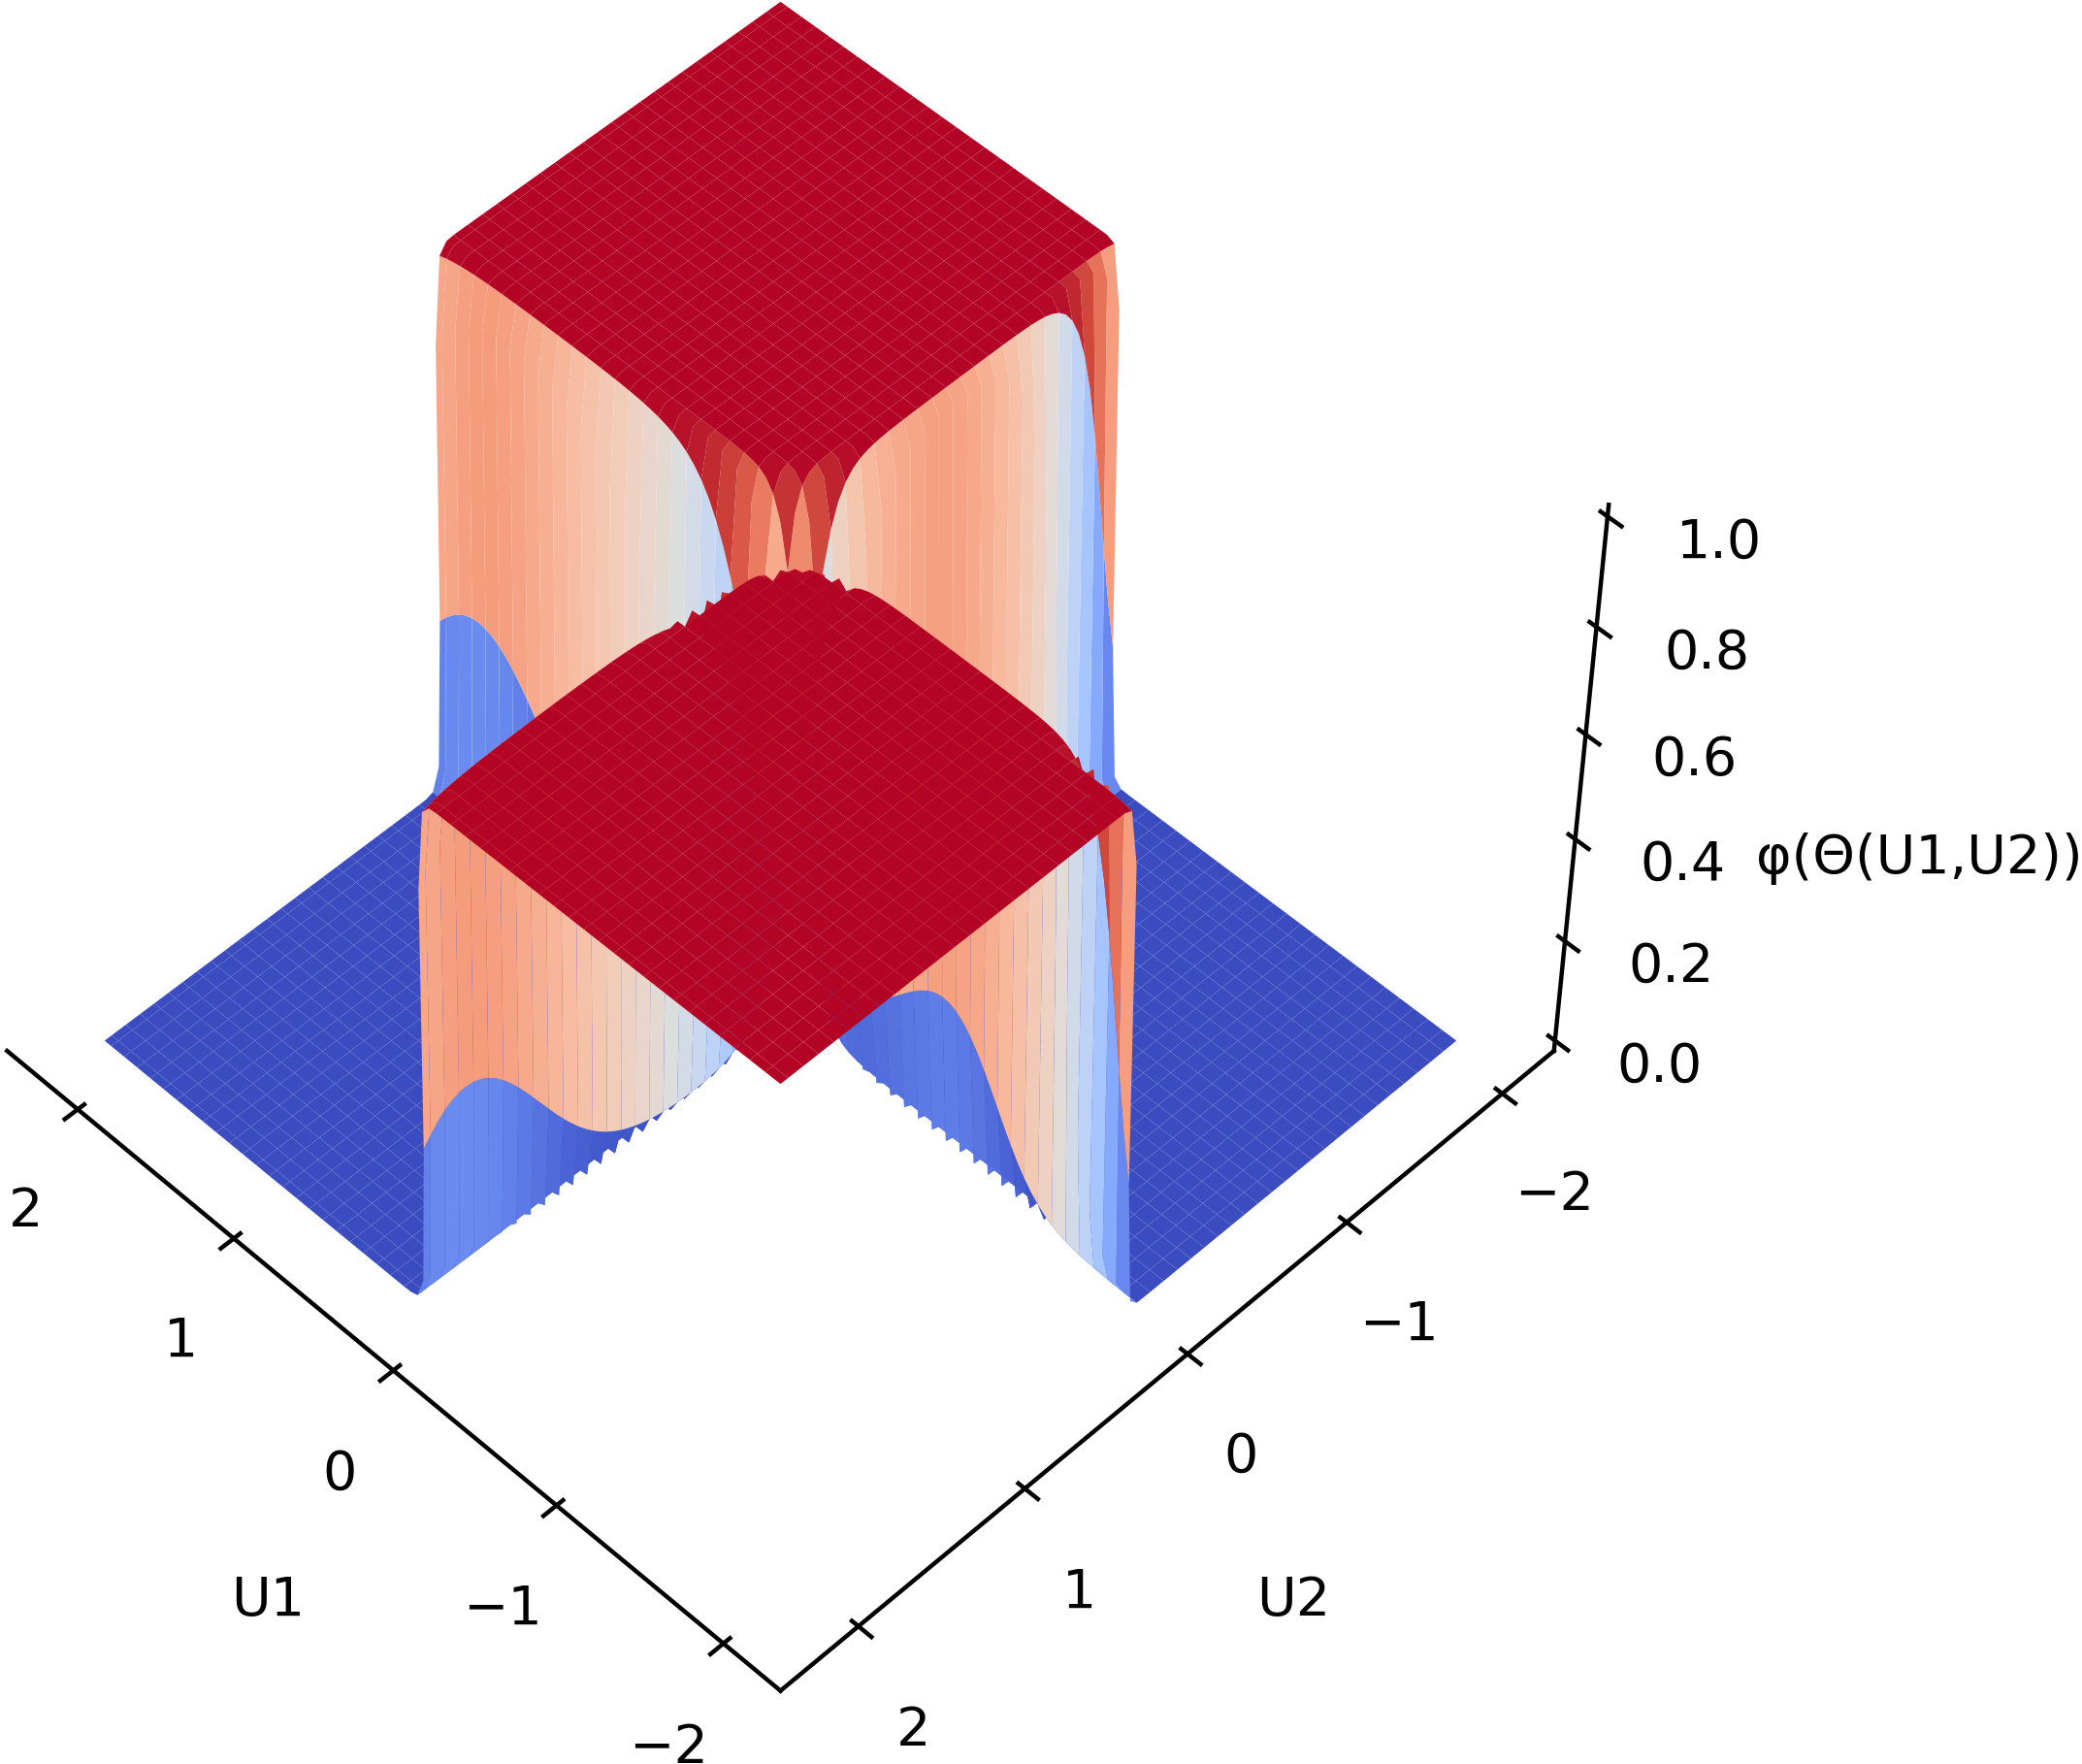
\includegraphics[width= 0.35\textwidth]{provengraphonnogrid}%
    \caption{From left to right: a bipartite graphon, a graph sampled from the bipartite graphon and the maximum a posteriori estimate of the graphon function by the RFM.}
    \label{estimatedbipartitegraphon}
\end{figure}

\begin{table}[h]
\caption{Mean $\pm$ Standard Deviation values for graph measures applied to sampled graphs from the predefined graphon (left column) and the estimated graphon (right column)}
\begin{tabular}{|l|l|l|l|}
\hline
 & \textbf{Predefined Graphon} & \textbf{Estimated Graphon}  \\ \hline
 Density & 0.503 $\pm$ 0.075 & 0.494 $\pm$ 0.012 \\ \hline
 Transitivity & 0.0 $\pm$ 0.0 & 0.019 $\pm$ 0.015 \\ \hline
Local Efficiency &  0.0 $\pm$ 0.0  & 0.064 $\pm$ 0.046 \\ \hline
Global Efficiency & 0.750 $\pm$ 0.055 & 0.746 $\pm$  0.006\\ \hline
Degree Assortativity Coefficient & N.a. $\pm$ N.a. &  -0.782 $\pm$ 0.250 \\ \hline
Average Clustering Coefficient & 0.0 $\pm$ 0.0 &  0.021 $\pm$ 0.017 \\ \hline
\end{tabular}
\end{table}

\subsection{Scale Free Graphon}
\begin{figure}[H]
    \center
    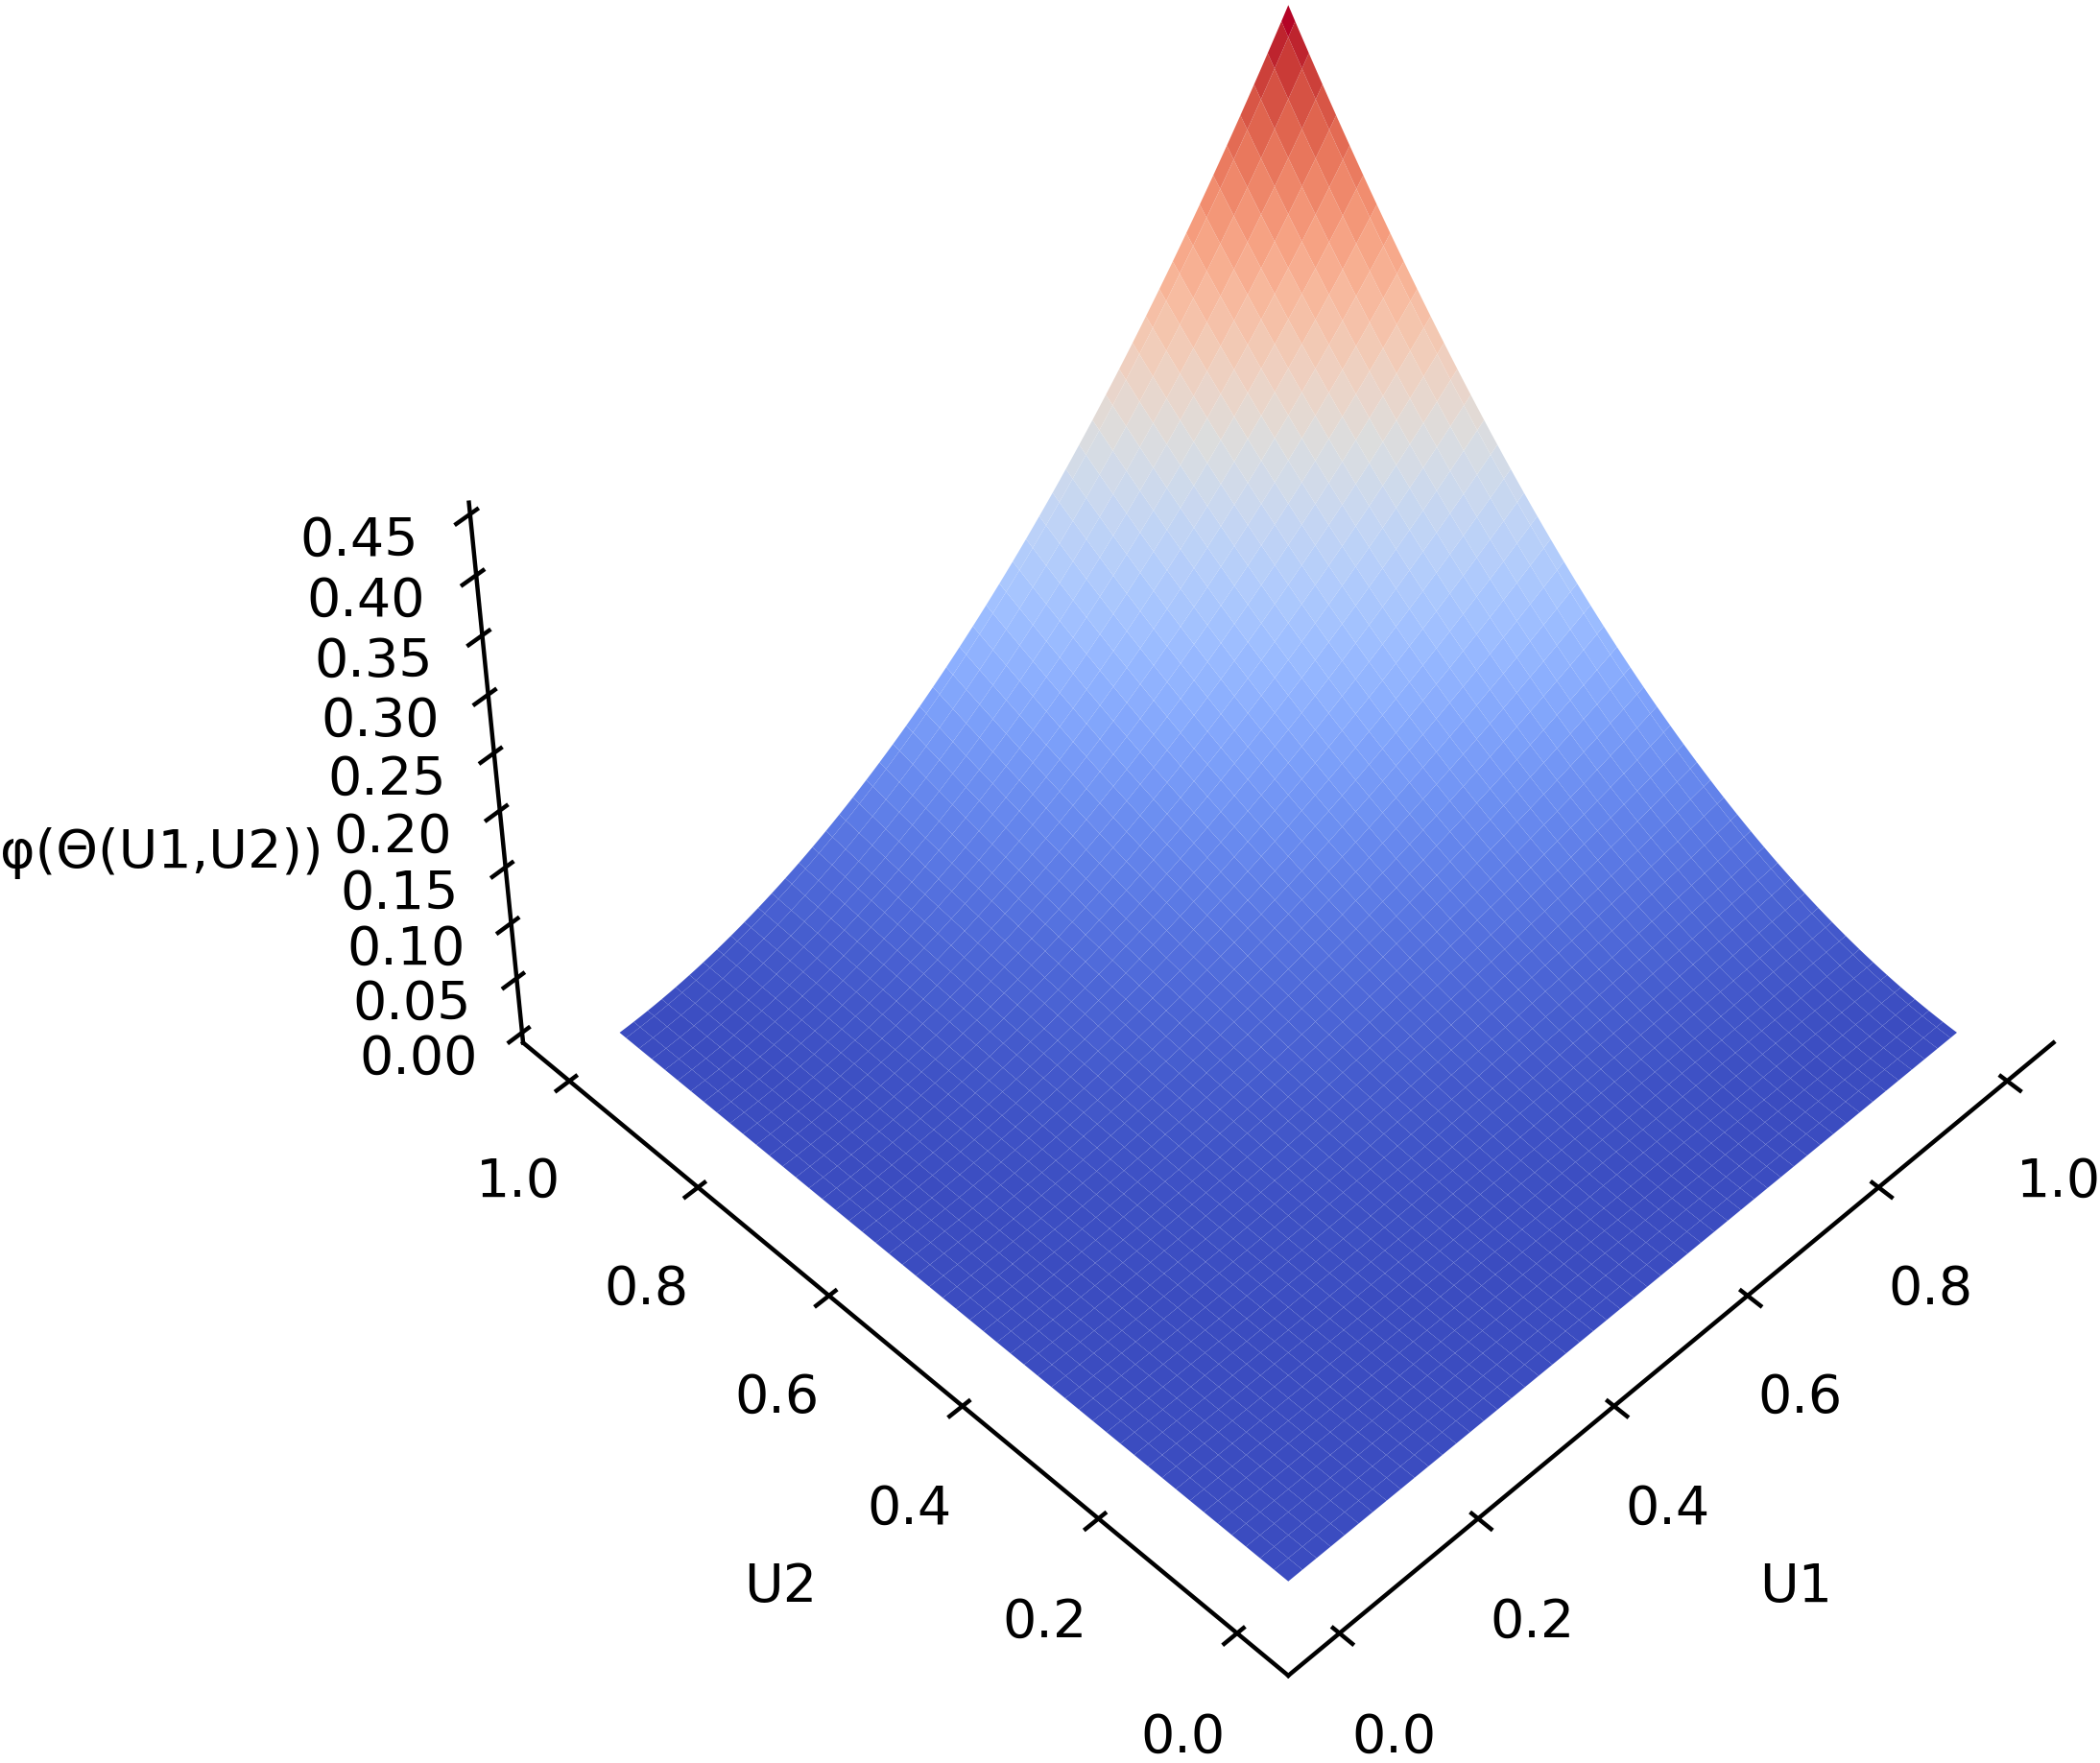
\includegraphics[width= 0.35\textwidth]{provengraphonscalefree}%
    \hfill
    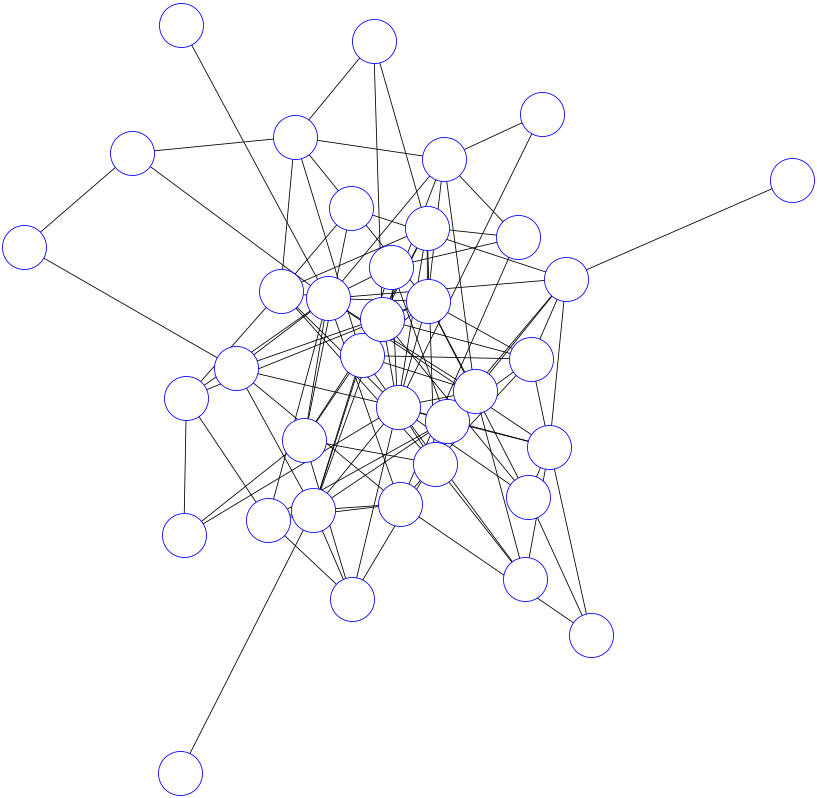
\includegraphics[width= 0.25\textwidth]{scalefreegraph}%
    \hfill
    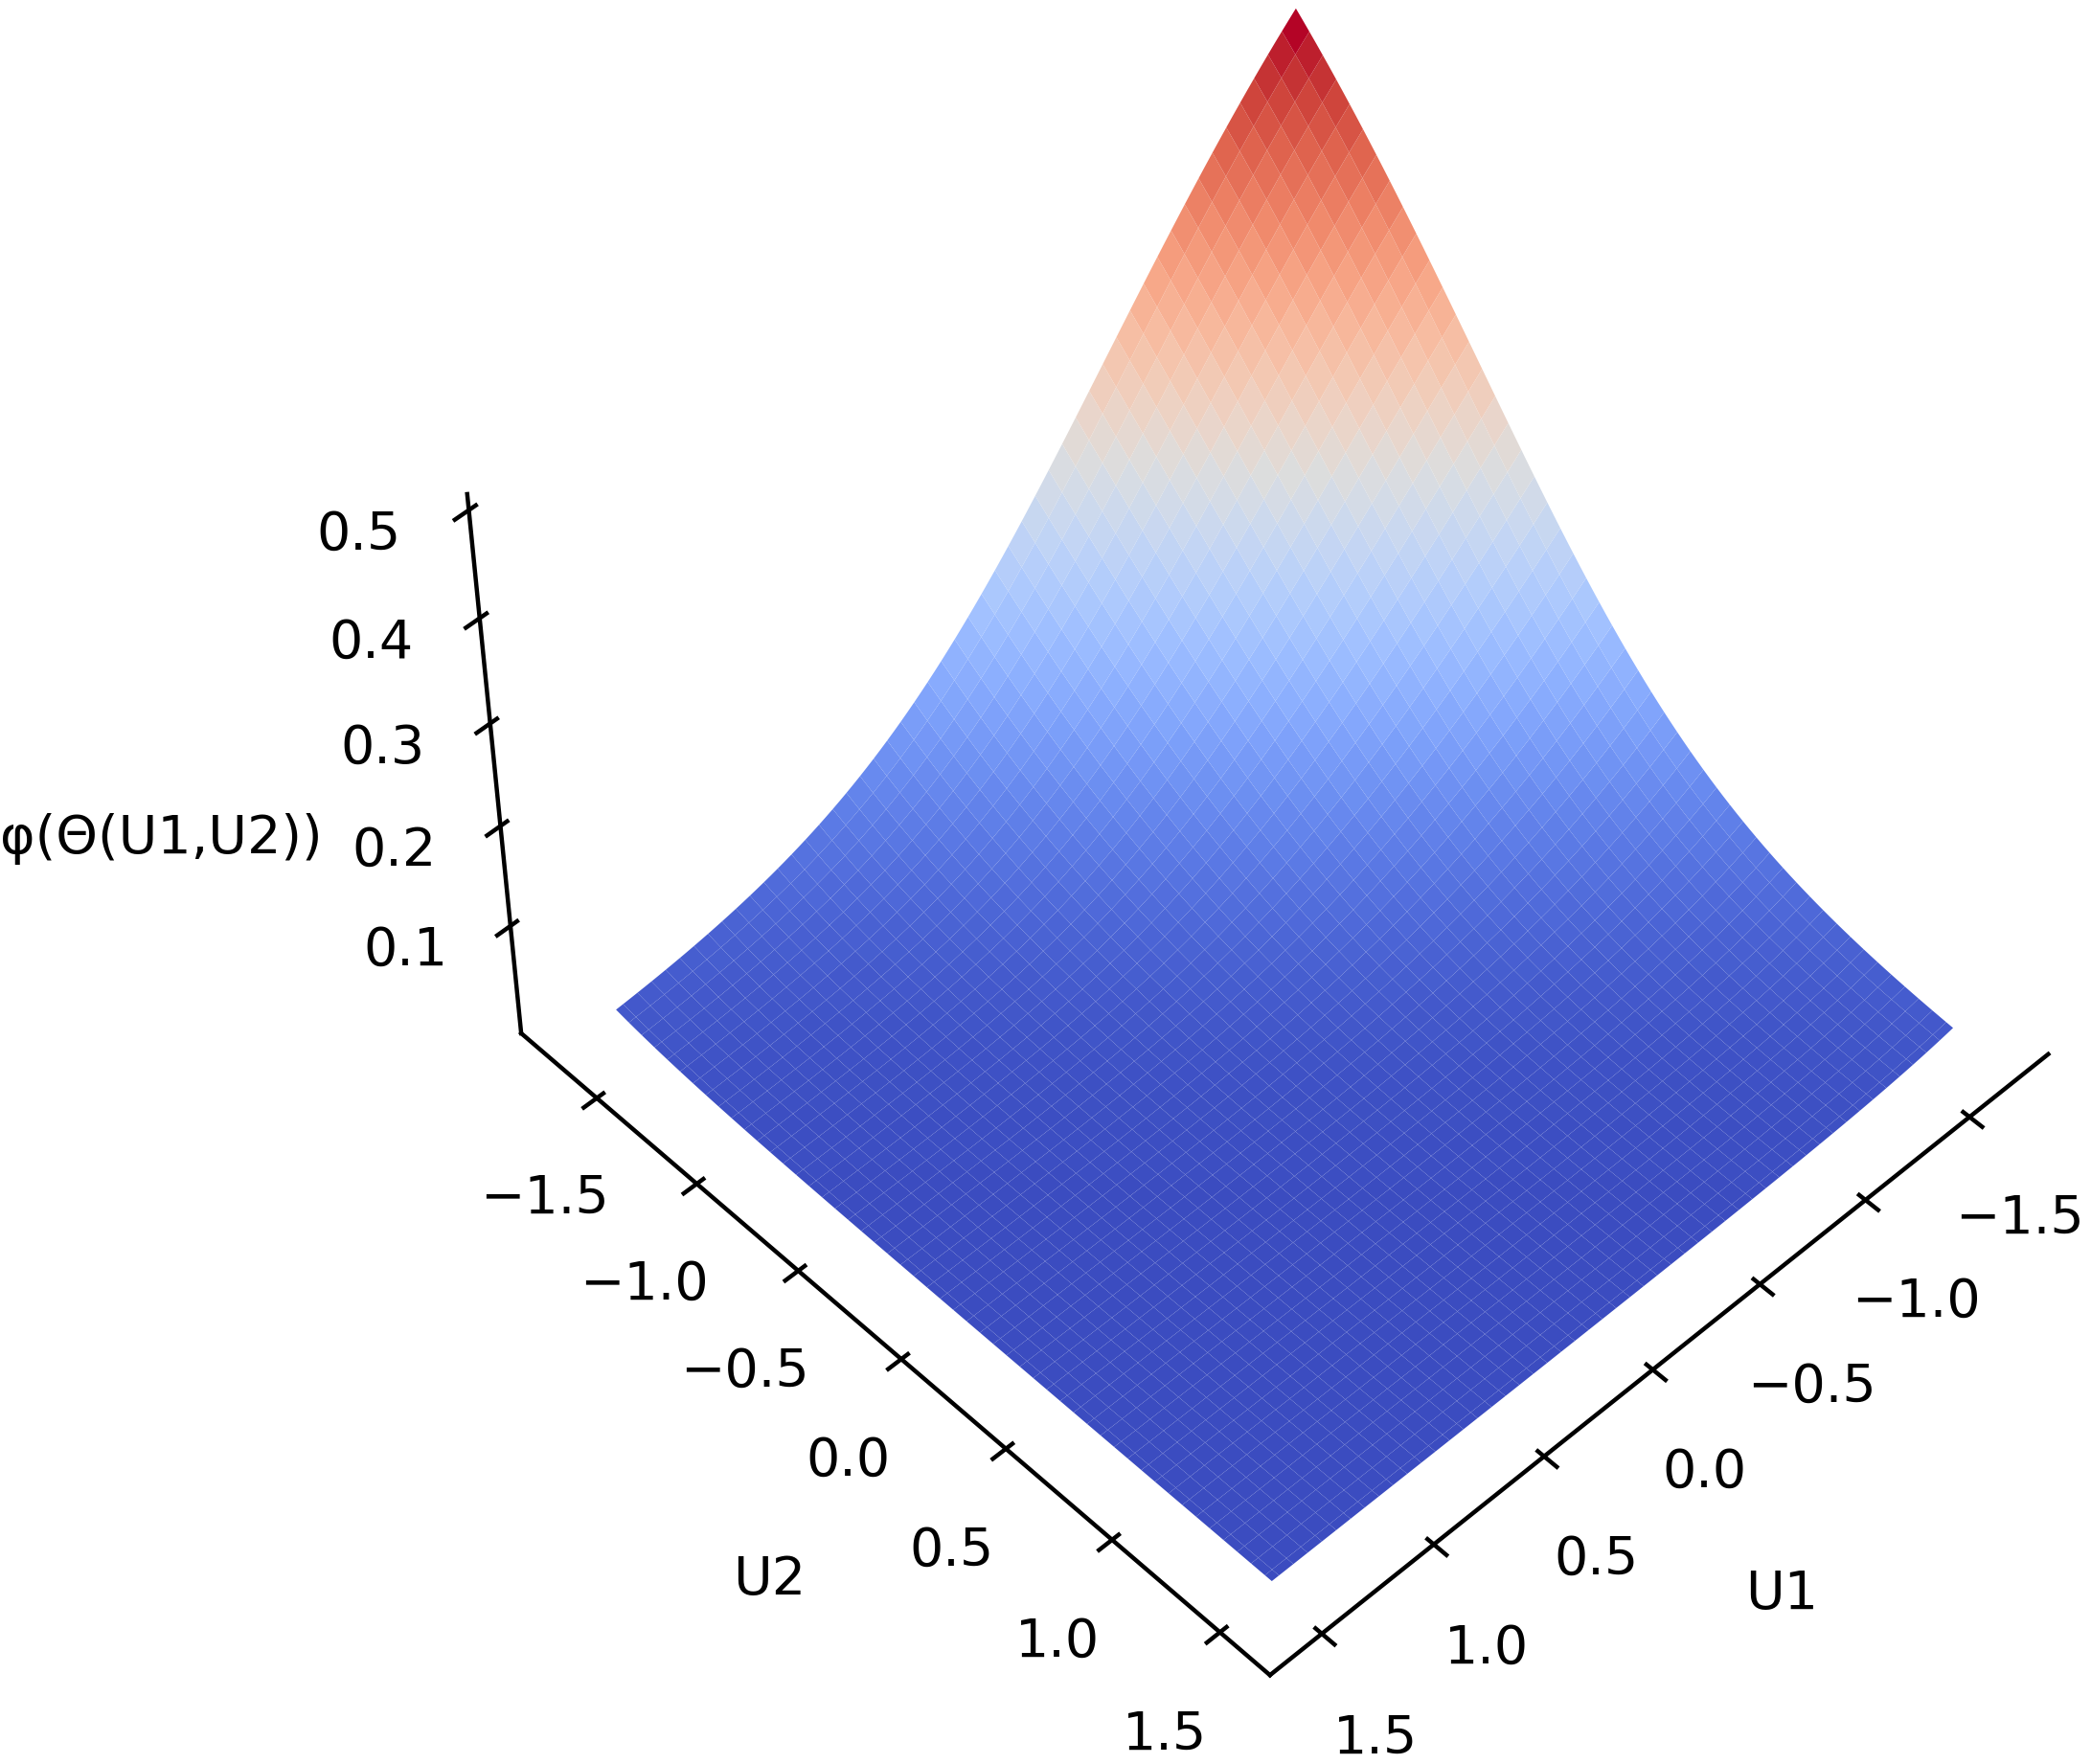
\includegraphics[width= 0.35\textwidth]{estimatedscalefreegraphon}%
    \caption{From left to right: a scale free graphon function, a graph sampled from the scale free graphon and the maximum a posteriori estimate of the graphon function by the RFM.}
    \label{estimatedscalefreegraphon}
\end{figure}
\begin{table}[h]
\caption{Mean $\pm$ Standard Deviation values for graph measures applied to sampled graphs from the predefined graphon (left column) and the estimated graphon (right column)}
\begin{tabular}{|l|l|l|l|}
\hline
 & \textbf{Predefined Graphon} & \textbf{Estimated Graphon}  \\ \hline
 Density & 0.051 $\pm$ 0.043 & 0.042 $\pm$ 0.012 \\ \hline
 Transitivity & 0.051 $\pm$ 0.176 & 0.110 $\pm$ 0.048 \\ \hline
Local Efficiency &  0.023 $\pm$ 0.078  & 0.083 $\pm$ 0.061 \\ \hline
Global Efficiency & 0.069 $\pm$ 0.074 & 0.173 $\pm$  0.058\\ \hline
Degree Assortativity Coefficient & N.a. $\pm$ N.a. &  -0.152 $\pm$ 0.139 \\ \hline
Average Clustering Coefficient & 0.023 $\pm$ 0.076 &  0.073 $\pm$ 0.050 \\ \hline
\end{tabular}
\end{table}
\subsection{Community Graphon}
\begin{figure}[H]
    \center
    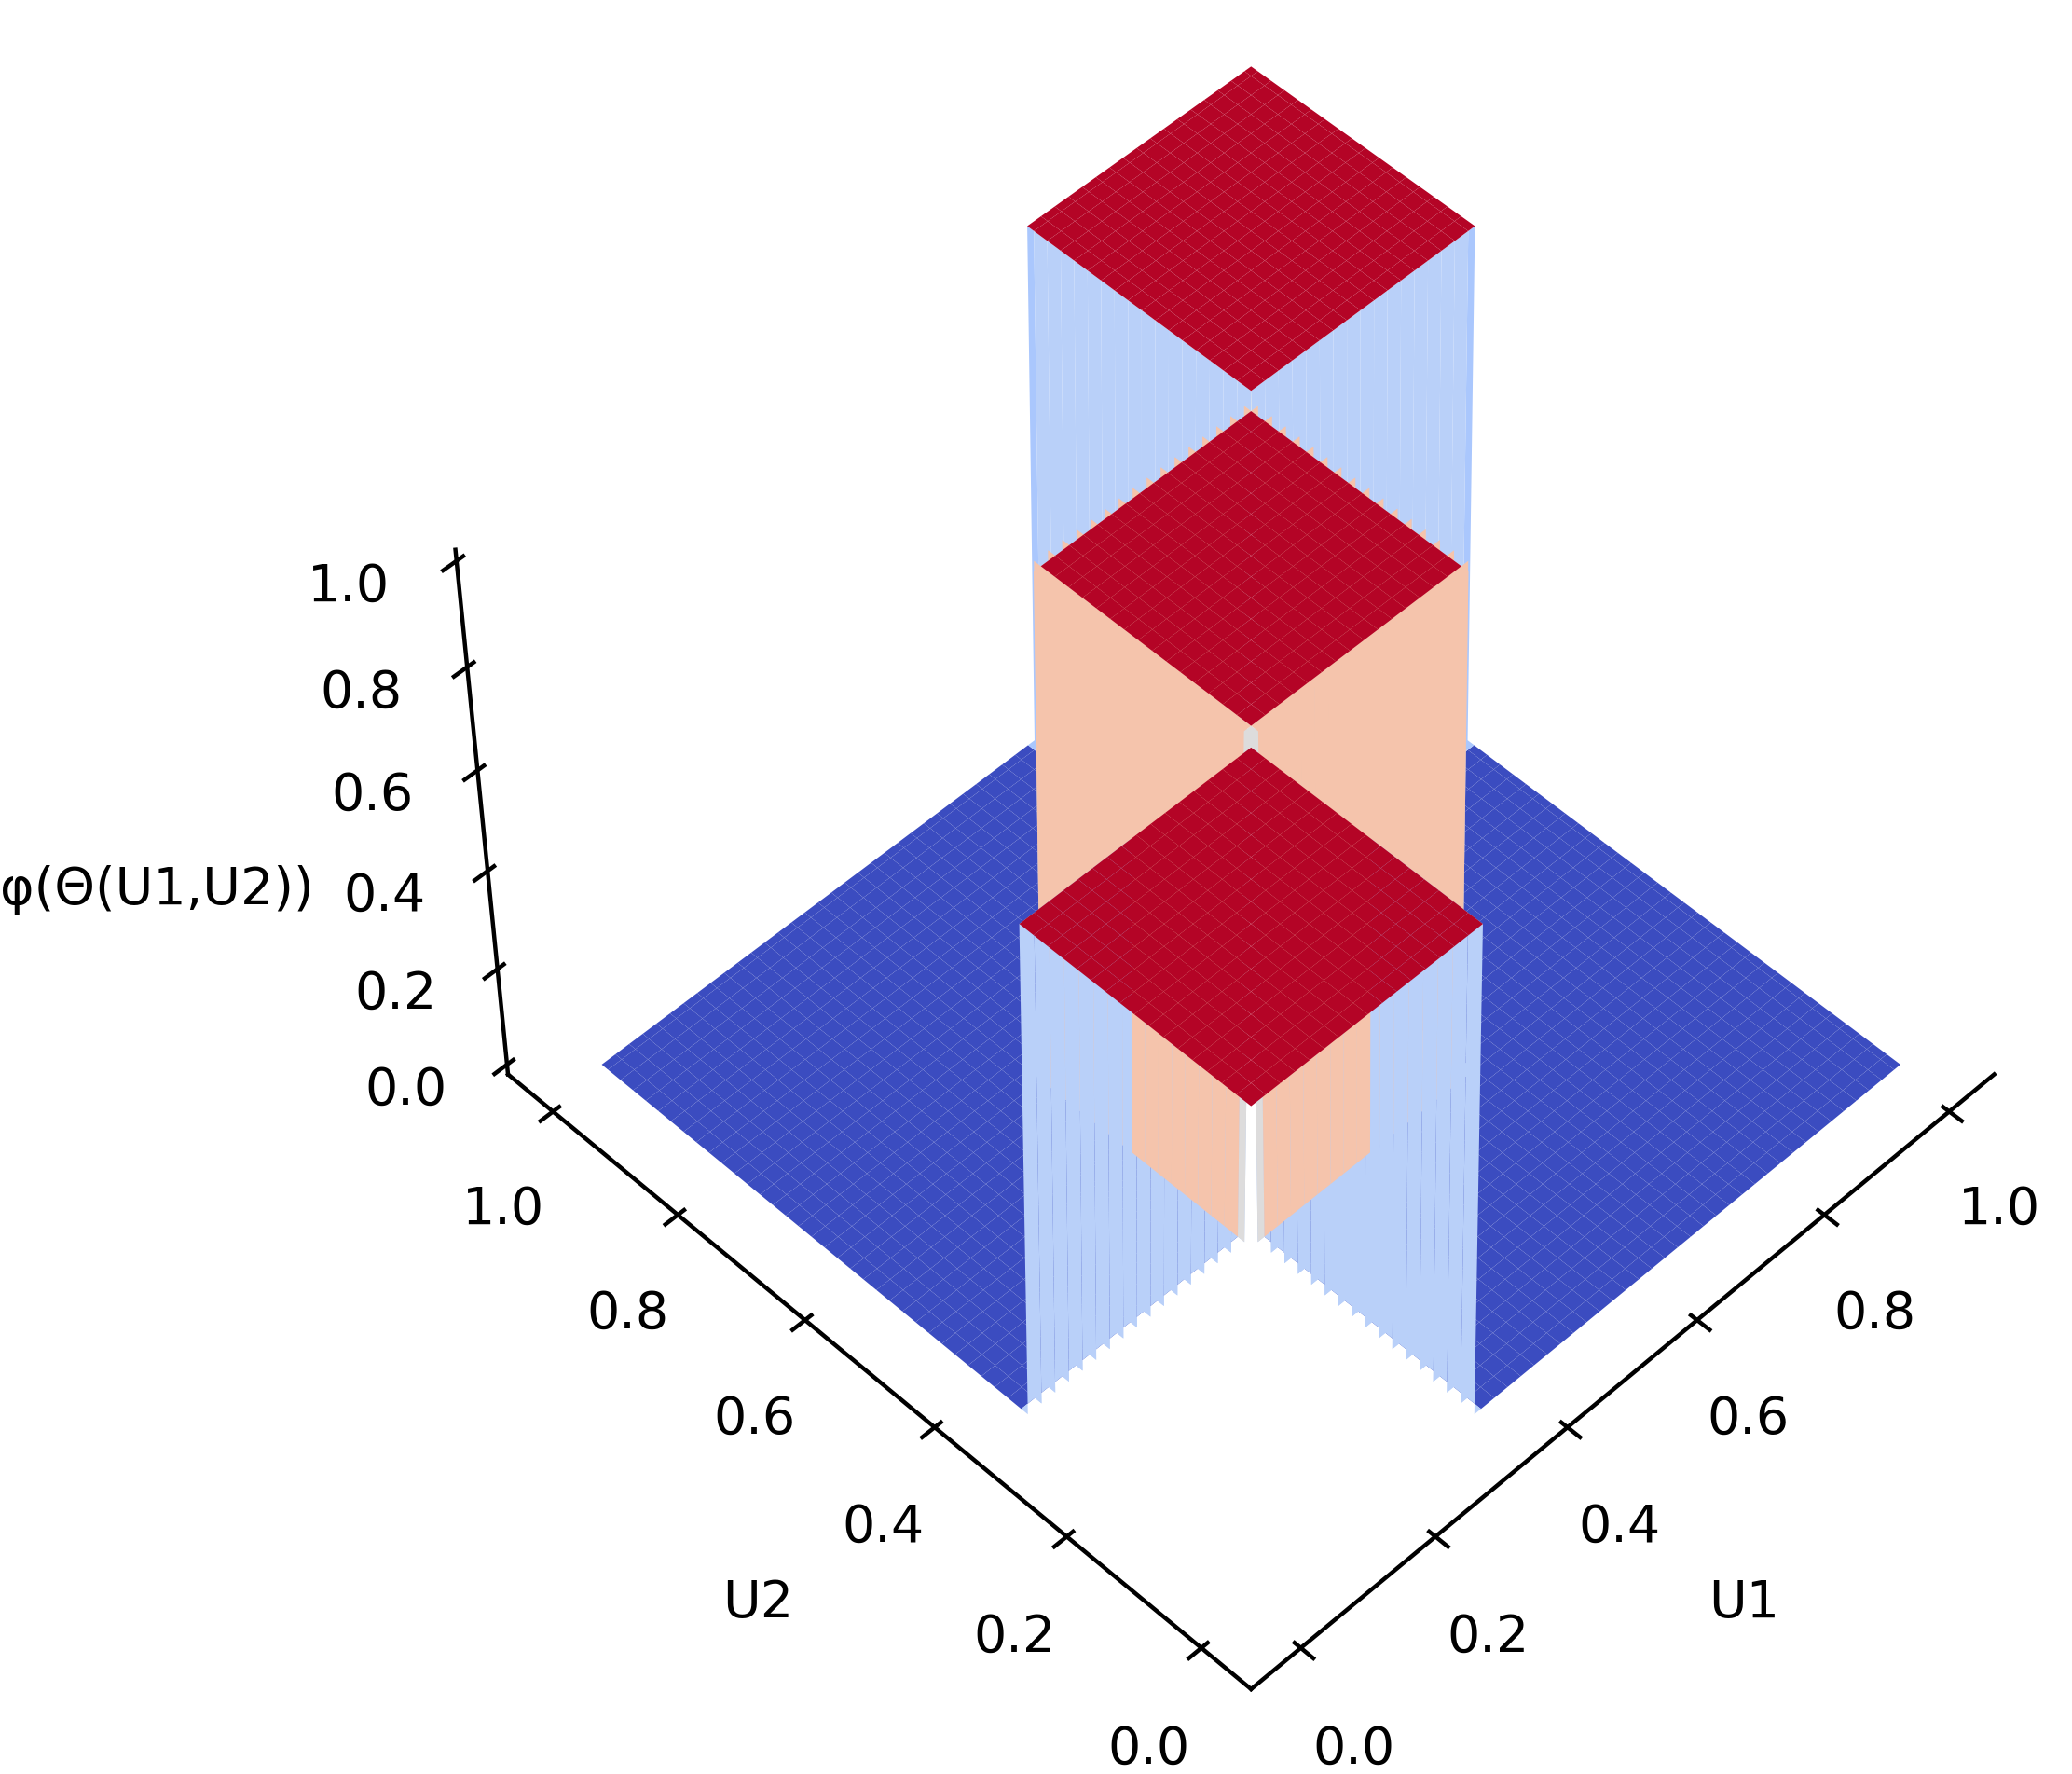
\includegraphics[width= 0.35\textwidth]{communitygraphon}%
    \hfill
    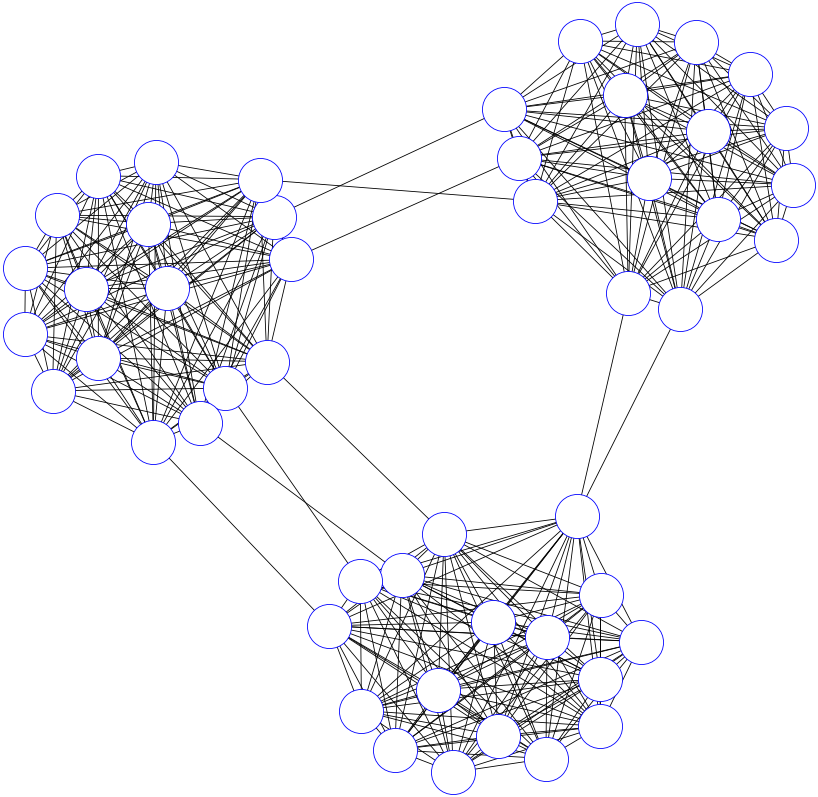
\includegraphics[width= 0.25\textwidth]{communitygraph}%
    \hfill
    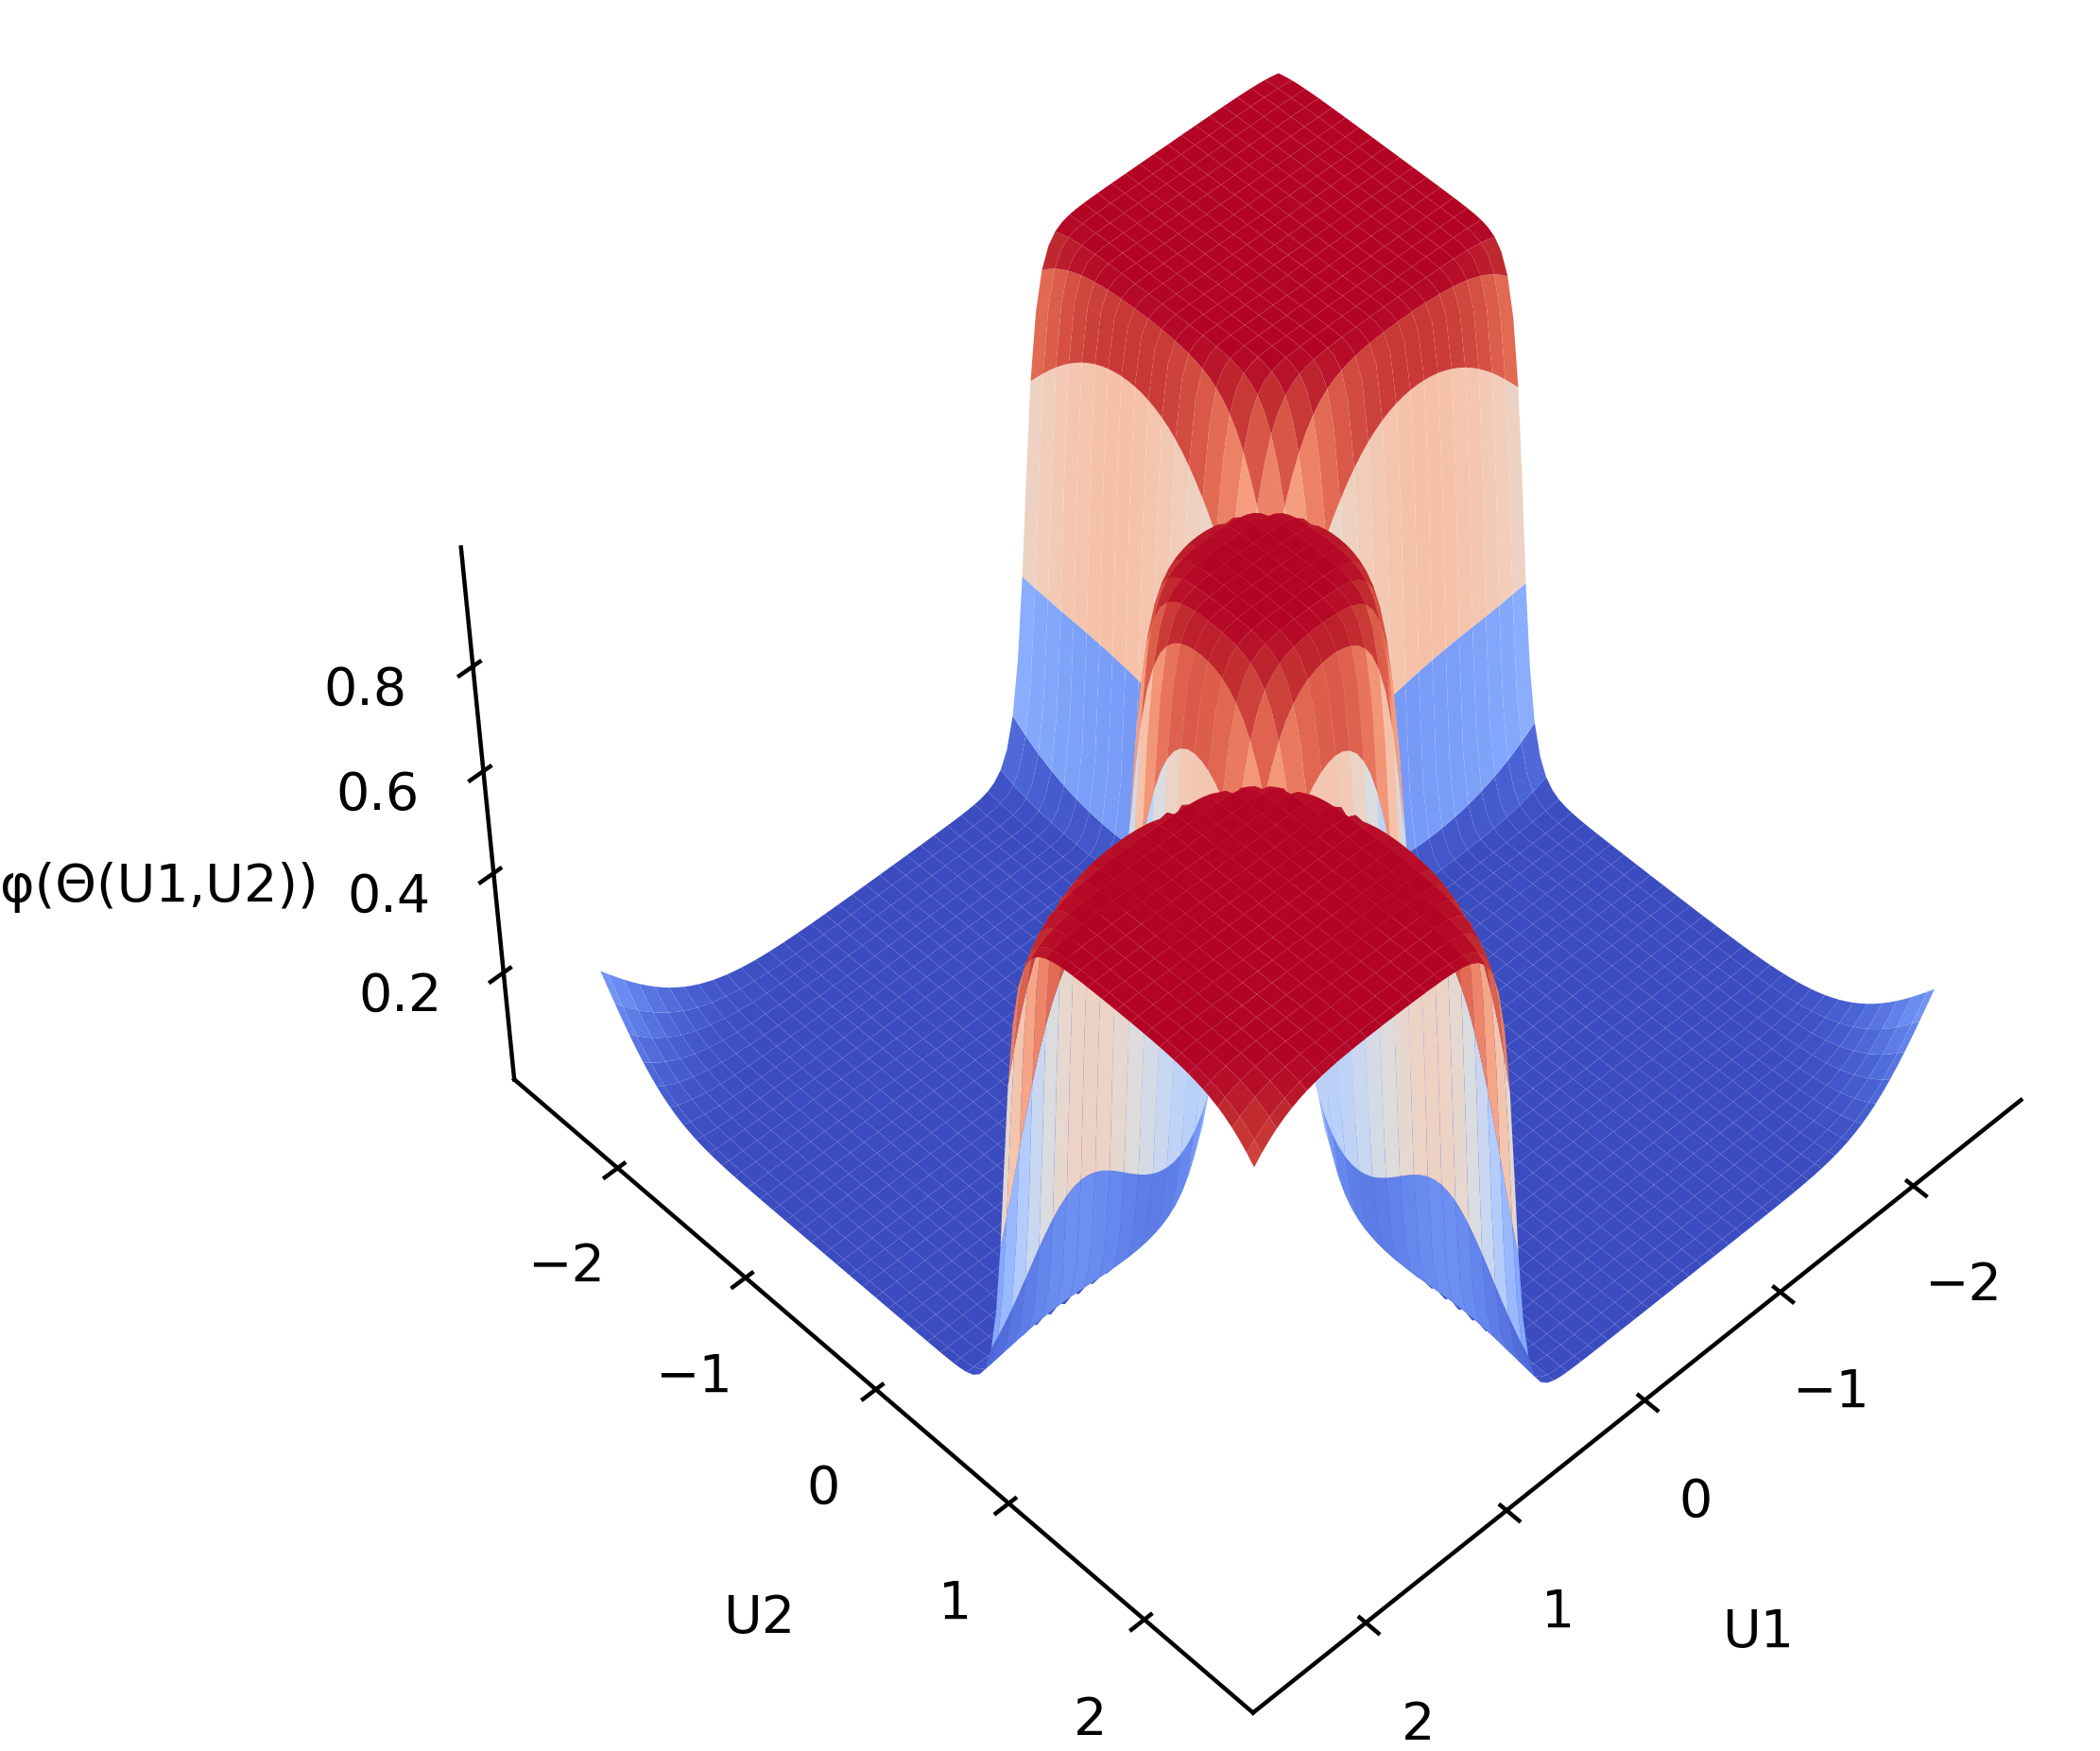
\includegraphics[width= 0.35\textwidth]{estimatedcommunitygraphon}%
    \caption{From left to right: a community graphon function, a graph sampled from the community graphon and the maximum a posteriori estimate of the graphon function by the RFM.}
    \label{estimatedcommunitygraphon}
\end{figure}
\begin{table}[h]
\caption{Mean $\pm$ Standard Deviation values for graph measures applied to sampled graphs from the predefined graphon (left column) and the estimated graphon (right column)}
\begin{tabular}{|l|l|l|l|}
\hline
 & \textbf{Predefined Graphon} & \textbf{Estimated Graphon}  \\ \hline
 Density & 0.338 $\pm$ 0.072                        & 0.397 $\pm$ 0.021 \\ \hline
 Transitivity & 0.981 $\pm$ 0.056                   & 0.779 $\pm$ 0.033 \\ \hline
Local Efficiency & 0.854 $\pm$ 0.113                & 0.898 $\pm$ 0.015 \\ \hline
Global Efficiency & 0.350$\pm$ 0.084 & 0.660 $\pm$ 0.017 \\ \hline
Degree Assortativity Coefficient & N.a. $\pm$ N.a. &  0.422 $\pm$ 0.154 \\ \hline
Average Clustering Coefficient & 0.854 $\pm$ 0.114 &  0.805 $\pm$ 0.029 \\ \hline
\end{tabular}
\end{table}
The above results show that the RFM can reliably learn connectomes. The visualisations show that the form of the predefined graphon functions was well estimated. For the community graphon however, the mean value for transitivity and global efficiency do not lie within the standard deviation of the mean of the graphs sampled from the predefined graphon. This indicates a mismatch of the estimated graphon with the actual graphon, which might be visible as a smaller middle structure in the graphon visualisation in figure \ref{estimatedcommunitygraphon}.
\section{Single Subject Link Prediction Comparison}
\label{singlelinkprediction}
\begin{table}[h]
\caption{Area under the receiver operator characteristic (AUROC) values for the RFM model on the MICA-MICs dataset.}
\begin{tabular}{|l|l|l|l|}
\hline
 & \textbf{RFM} & \textbf{missSBM} & \textbf{eigenmodel}  \\ \hline
 MICA-MICs & 0.88 $\pm$ 0.004 & 0.855 $\pm$ 0.0 & 0.854 $\pm$ 0.001  \\ \hline
\end{tabular}
\end{table}
\noindent
The results of the single link prediction showed as expected that the RFM improves upon models that it generalises, such as the missSBM and the eigenmodel. It is noteworthy however, that the standard deviation of AUROC values is small. This is most likely due to the thresholded tractograms becoming very similar, as they have been downsampled using consistency thresholding.
% \section{Group Link Prediction Comparison}
% \begin{table}[H]
% \begin{tabular}{|l|l|l|l|l|}
% \hline
% Group Size & 1 & 2 & 3 & 4 \\ \hline
% Mean & 0.85 &  &  &  \\ \hline
% Standard Deviation & &  &  &  \\ \hline
% \end{tabular}
% \caption{Area under the receiver operator characteristic (AUROC) values for the RFM model trained on one complete subject graph and one partial subject graph, predicting the held out edges of the second graph.}
% \end{table}

\section{Connectome Sample Quality}
\label{connectomesamplequaliyresults}
\begin{figure}[H]
    \center
    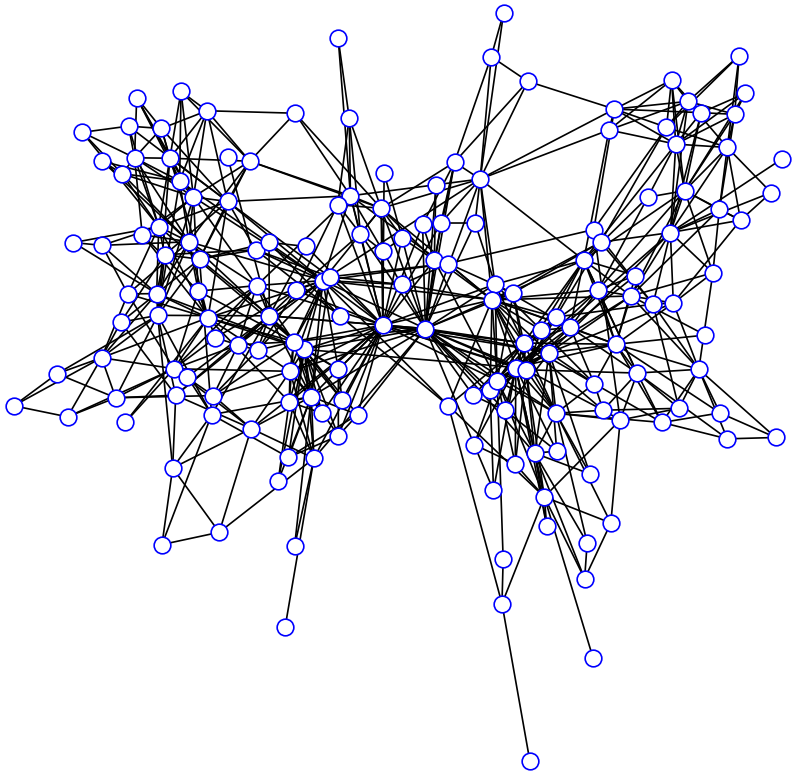
\includegraphics[width= 0.4\textwidth]{subject_graph}%
    \hfill
    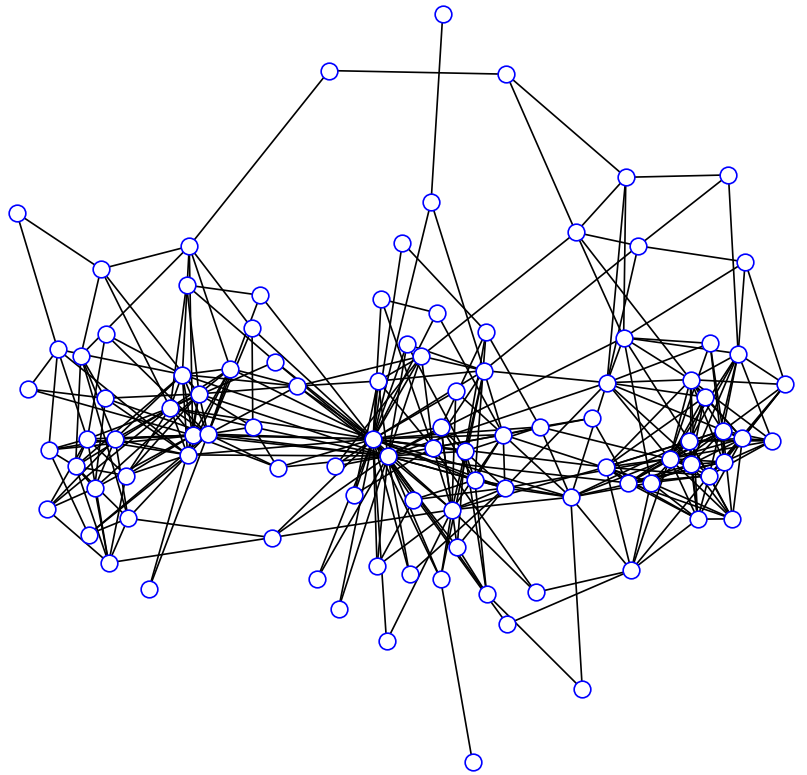
\includegraphics[width= 0.4\textwidth]{sampled_graph}%
    \caption{The thresholded graph of a subject from the HCP data (left) and a graph sampled from the mean posterior graphon function (right).}
\end{figure}
\begin{table}[h]
\caption{Graph properties for the MICA-MICs dataset after thresholding and average graph properties for graphs sampled from graphon estimates based on the MICA-MICs dataset.}
\begin{tabular}{|l|l|l|l|}
\hline
 & \textbf{Thresholded MICA-MICs} & \textbf{Sampled Graphs}  \\ \hline
Density           & 0.200 $\pm$ 0.000  & 0.091 $\pm$ 0.0187\\ \hline
Transitivity      & 0.019 $\pm$ 0.015  & 0.318 $\pm$ 0.094\\ \hline
Local Efficiency  & 0.756 $\pm$ 0.000  & 0.494 $\pm$ 0.146 \\ \hline
Global Efficiency & 0.556 $\pm$ 0.000  & 0.437 $\pm$ 0.085\\ \hline
Degree Assortativity Coefficient  & -0.039 $\pm$ 0.001 & - 0.093 $\pm$ 0.325\\ \hline
Average Clustering Coefficient    & 0.541 $\pm$ 0.001  &  0.352 $\pm$ 0.112 \\ \hline
\end{tabular}
\end{table}
\section{Graphon Based Graph Comparison}
\begin{table}[H]
\centering
\caption{Graph attributes for the original subject graph and averaged for samples from the RFM model fitted to the subject graph.}
\label{graphcomparison}
\begin{tabular}{|l|l|l|l|}
\hline
& \textbf{Desikan \& Killiany 100} & \textbf{Vos de Wael 200} & \textbf{Distance} \\ \hline
Graph Density                    & 0.200   & 0.200  & 0.000 \\ \hline
Transitivity                     & 0.448   & 0.438  & 0.010 \\ \hline
Local Efficiency                 & 0.756   & 0.746  & 0.010 \\ \hline
Global Efficiency                & 0.557   & 0.575  & 0.018 \\ \hline
Degree Assortativity Coeff. & -0.039  & -0.026 & 0.013 \\ \hline
Average Clustering Coeff.  & 0.542   & 0.513  & 0.029 \\ \hline
\end{tabular}
\end{table}
\begin{table}[H]
\centering
\caption{Graph attributes for samples drawn from the graphon estimated for the Desikan \& Killiany 100 parcellation (RFM$_{100}$) and for Vos de Wael 200 (RFM$_{200}$).} 
\label{samplecomparison}
\begin{tabular}{|l|l|l|l|}
\hline
& \textbf{RFM$_{100}$} & \textbf{RFM$_{200}$} & \textbf{Distance} \\ \hline
Graph Density               & 0.285  $\pm$ 0.019  & 0.346 $\pm$ 0.036   & 0.061 $\pm$ 0.041   \\ \hline
Transitivity                & 0.501  $\pm$ 0.023  & 0.579 $\pm$ 0.032   & 0.078 $\pm$ 0.039  \\ \hline
Local Efficiency            & 0.758  $\pm$ 0.020  & 0.800 $\pm$ 0.020   & 0.042 $\pm$ 0.028  \\ \hline
Global Efficiency           & 0.637  $\pm$ 0.012  & 0.664 $\pm$ 0.019   & 0.027 $\pm$ 0.022  \\ \hline
Degree Assortativity Coeff. & -0.055 $\pm$ 0.042  & -0.056 $\pm$ 0.067  & 0.001 $\pm$ 0.079  \\ \hline
Average Clustering Coeff.   & 0.541  $\pm$ 0.026  & 0.609 $\pm$ 0.028   & 0.068 $\pm$ 0.038  \\ \hline
\end{tabular}
\end{table}

Two tractograms from a single subject, but with different parcellations were chosen from the MICA-MICs dataset. Parcellation Desikan \& Killiany 100 has 86 regions of interest, while Vos de Wael 200 has 216 regions of interest. In table \ref{graphcomparison}, six different graph measures were applied to both graphs and the distance between the result was noted. 
\section{Visualisation}
\begin{figure}[H]
    \center
    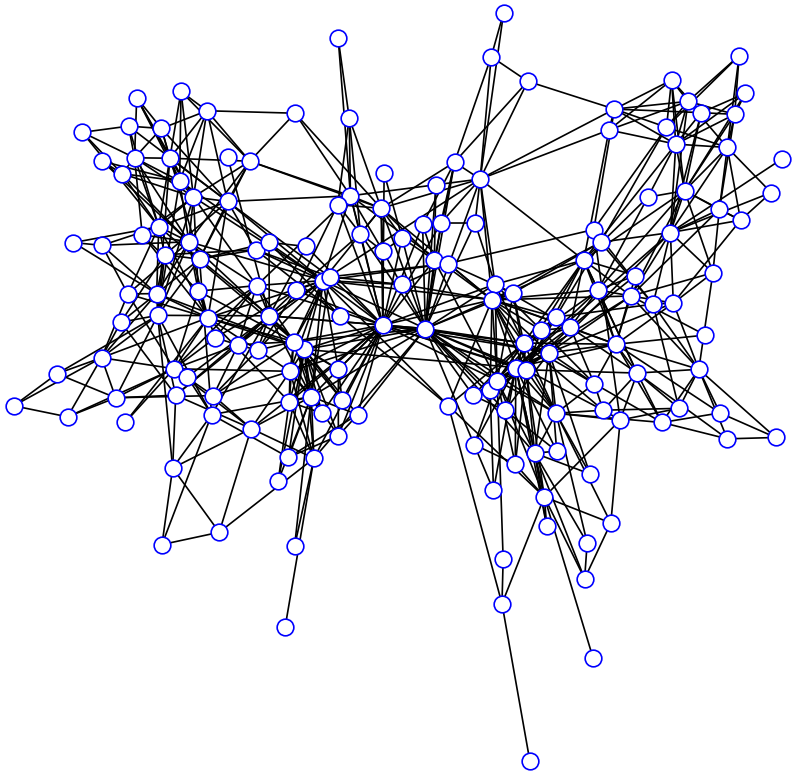
\includegraphics[width= 0.25\textwidth]{subject_graph}%
    \hfill
    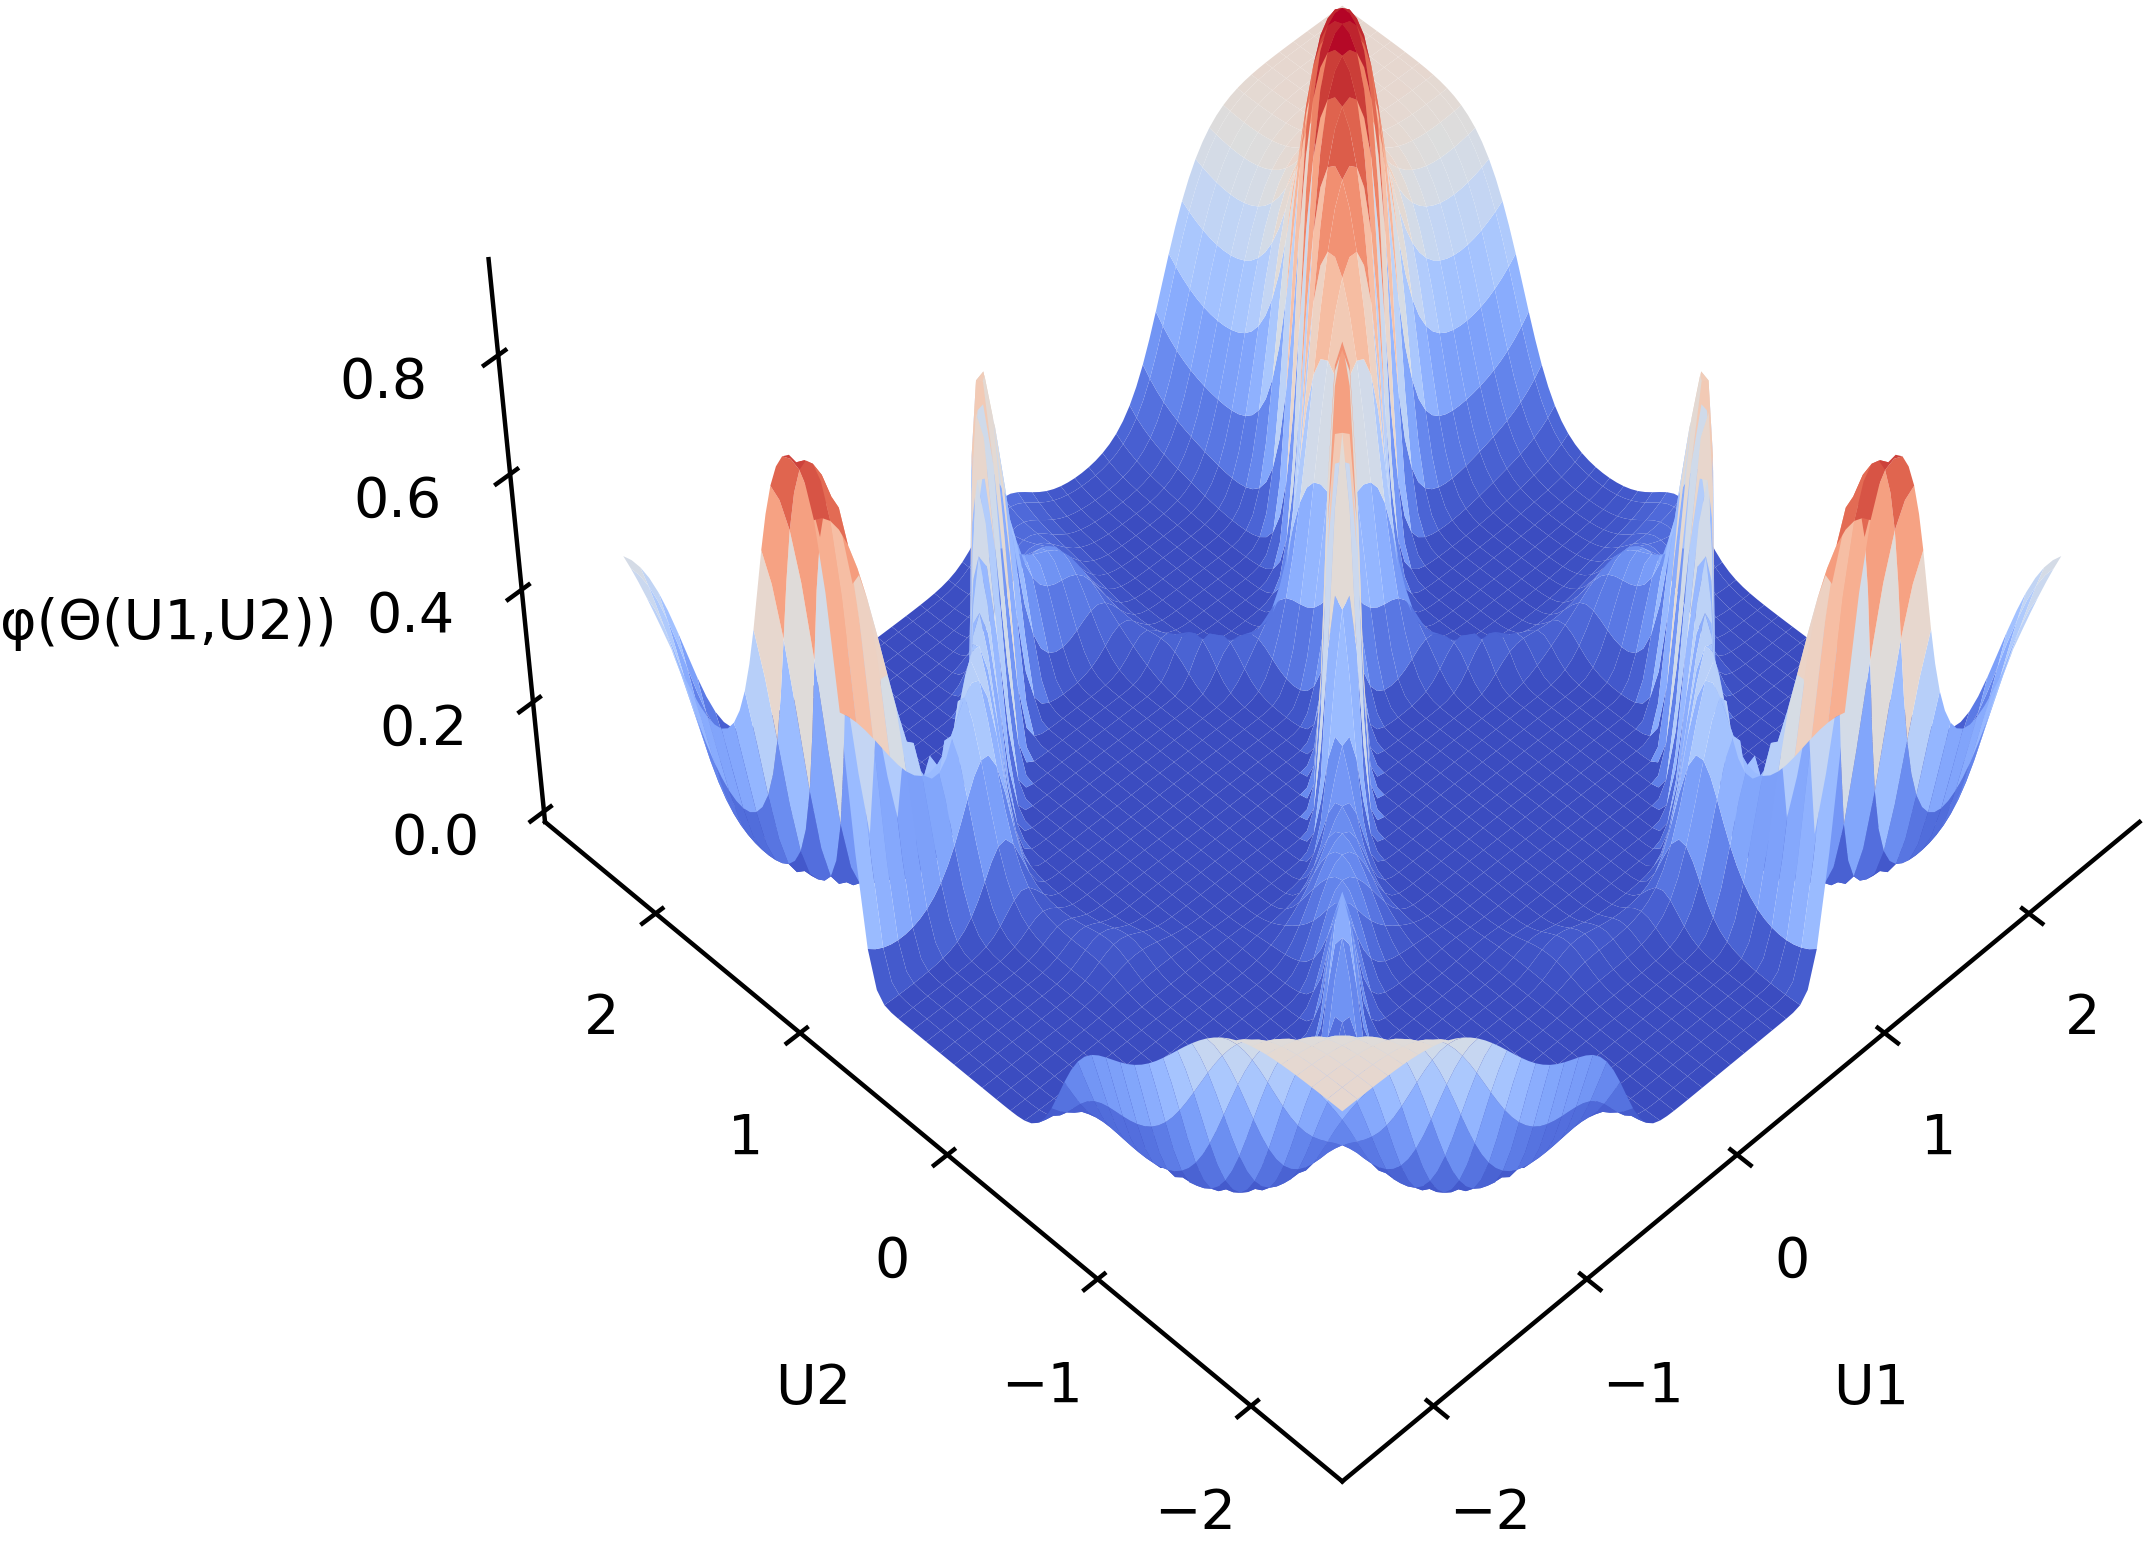
\includegraphics[width= 0.4\textwidth]{graphon_100307}%
    \hfill
    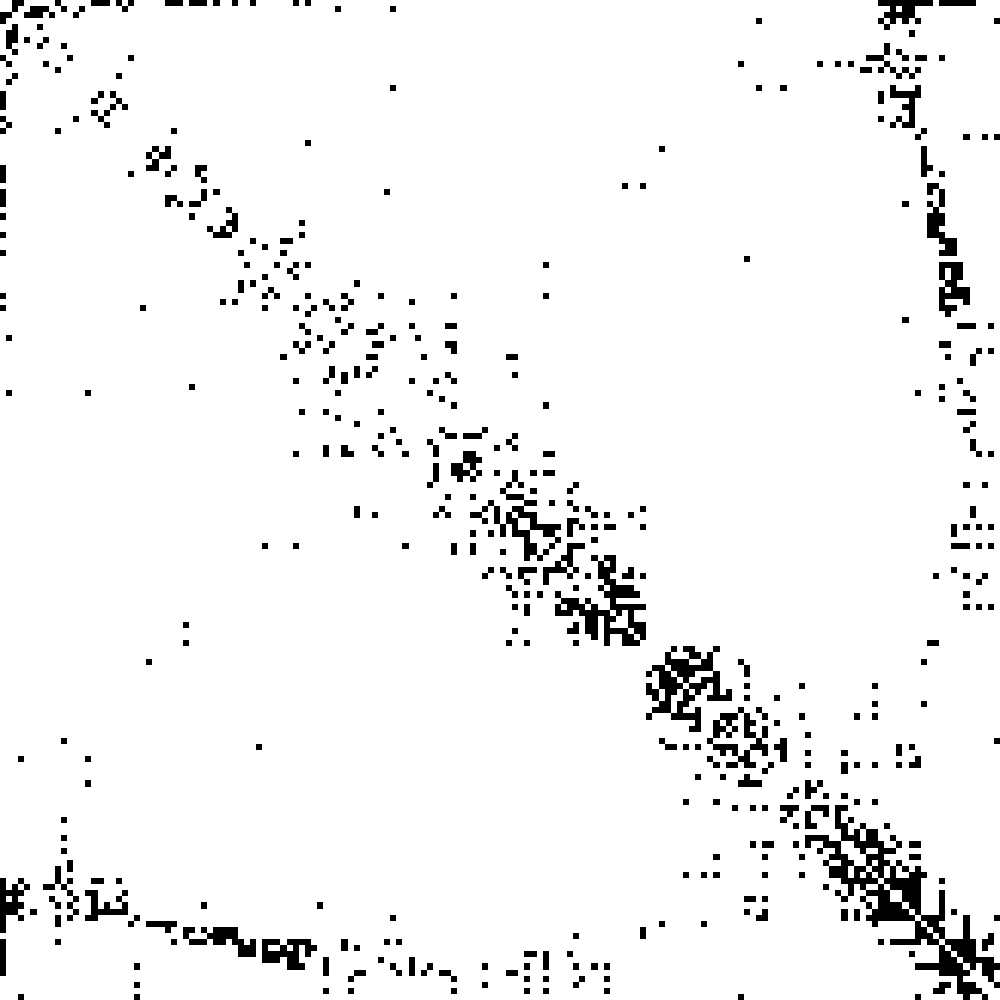
\includegraphics[width= 0.25\textwidth]{eldrichgod}%
    \caption{From left to right: The structural connectivity graph of a HCP subject, graphon function maximum a posteriori RFM estimate, adjacency matrix rearranged using the latent node positions estimates of the RFM.}
    \label{visualisation 1}
\end{figure}
The graphon function is hard to interpret, as it is in fact a more complex object than a single graph is. Furthermore, the same graphon was estimated again, which resulted in a different graphons visible in figure \ref{alternativegraph}. The adjacency matrix sorted by the maximum a posteriori estimate of the latent node positions might be more meaningful however. As \citeA{lloyd2012} explain, that many edges near the diagonal express a sense of homophily, which is actually expected of brain networks \cite{larivi2019} and it is visible in the sorted adjacency matrix on the right.

\begin{figure}[H]
    \center
    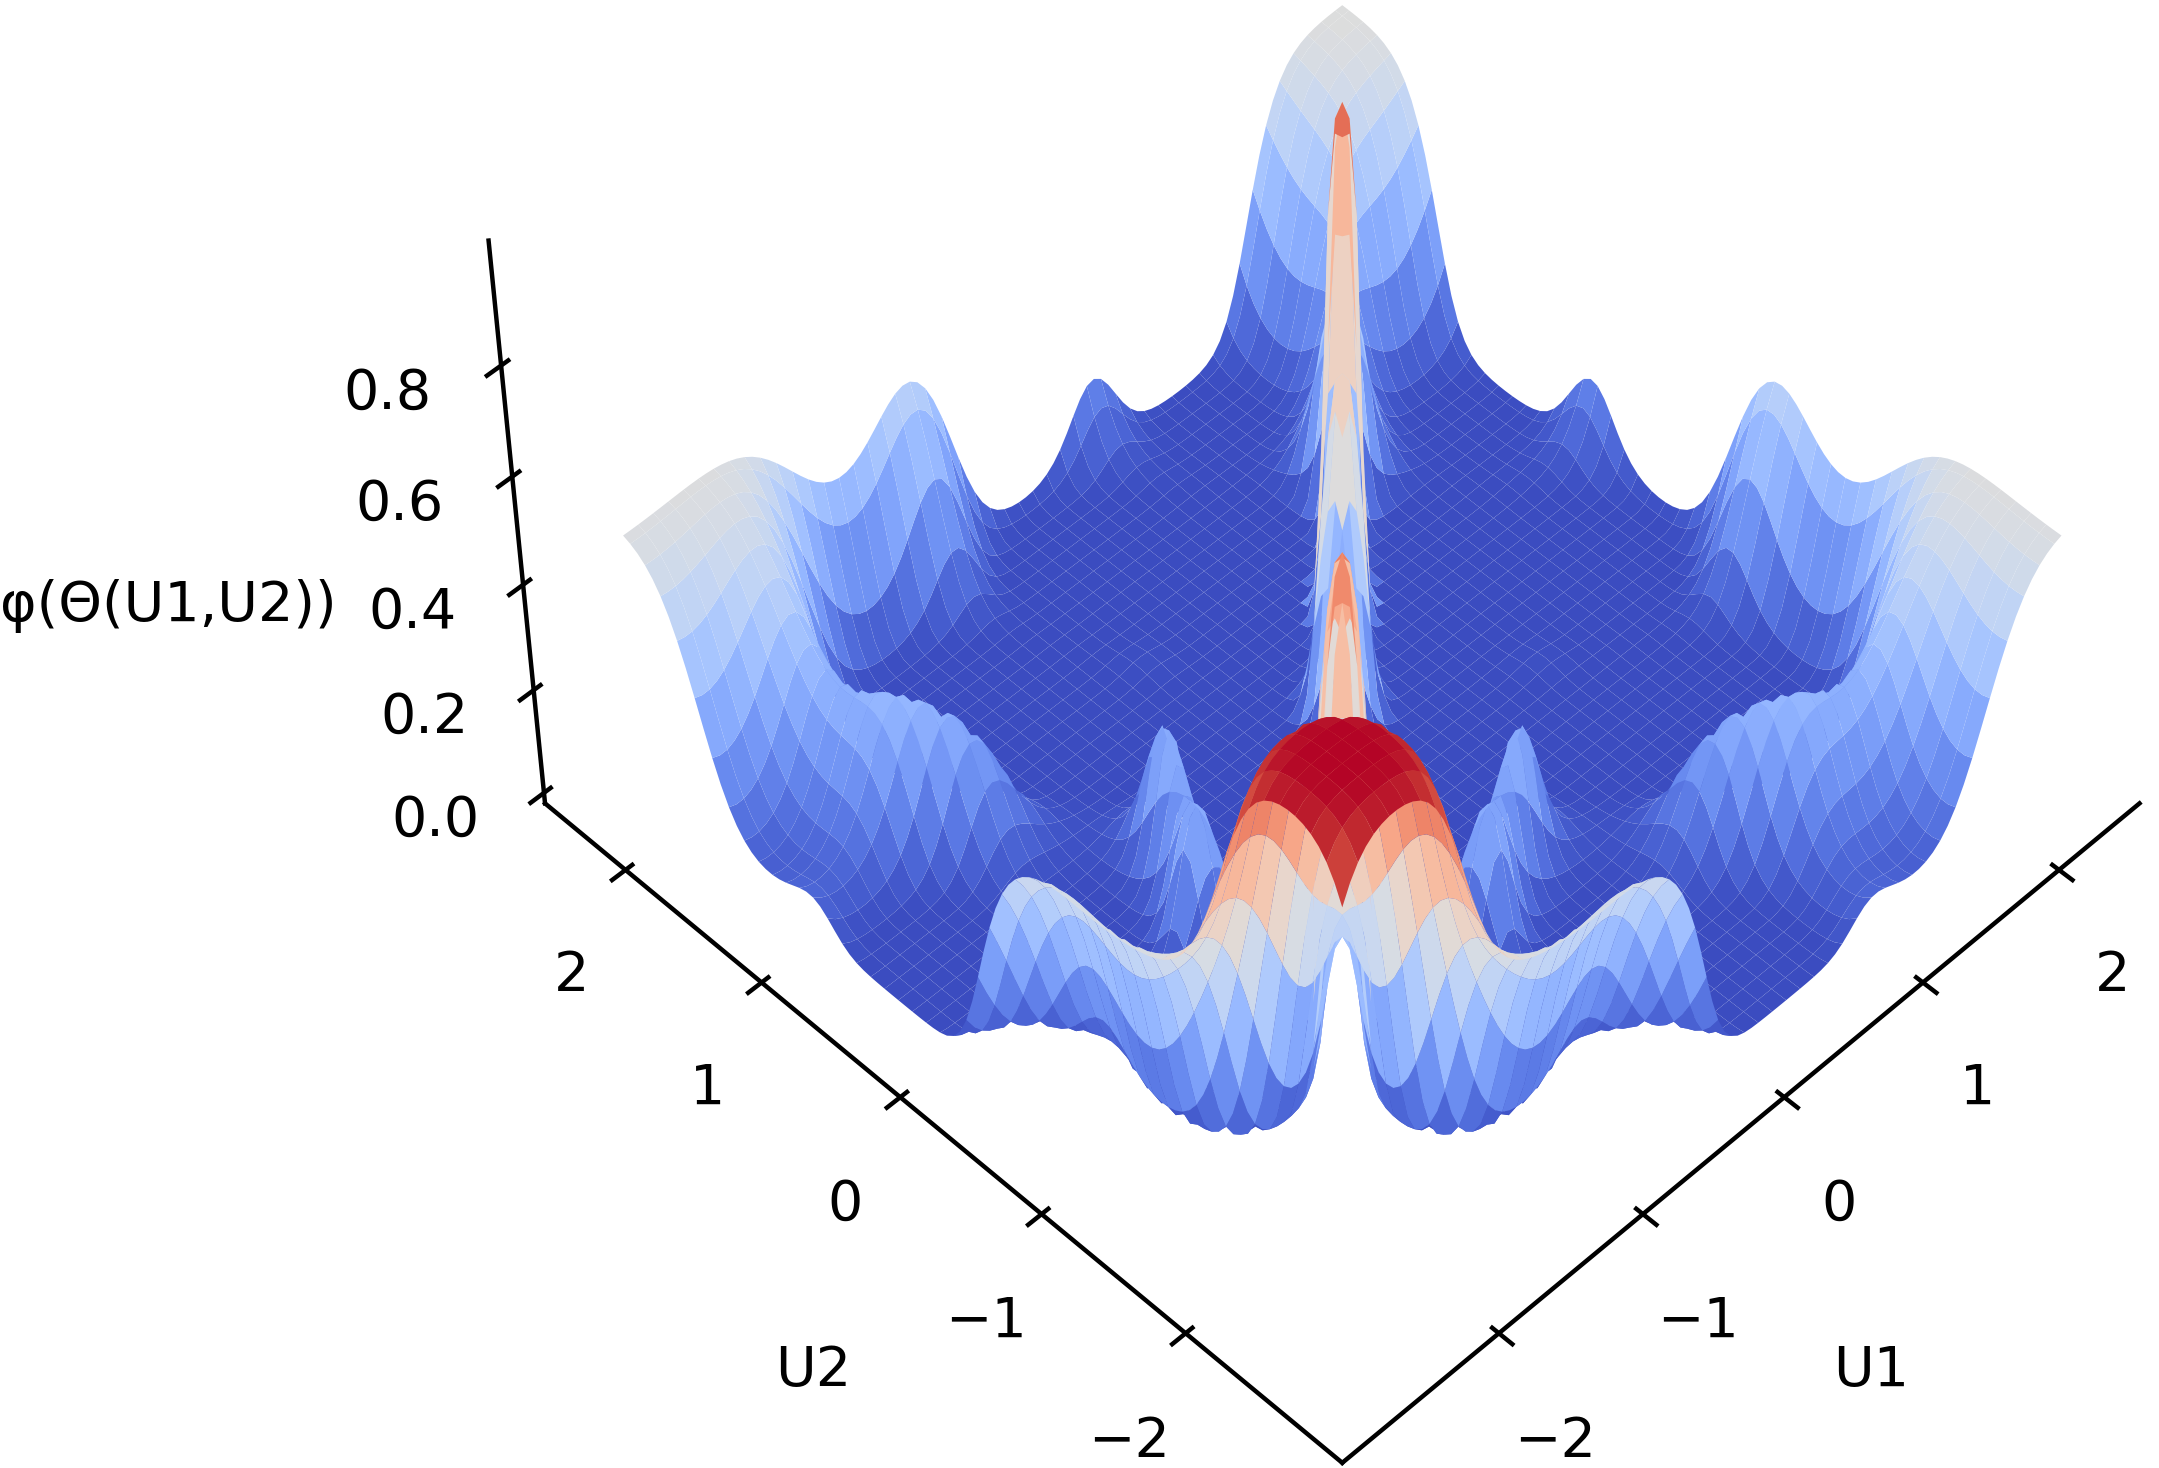
\includegraphics[width= 0.6\textwidth]{graphon_100307_2}%
    \hfill
    \caption{A graph estimated for the same observed network as the graphon estimation in figure \ref{visualisation 1}}
    \label{alternativegraph}
\end{figure}

\begin{figure}[H]
    \center
    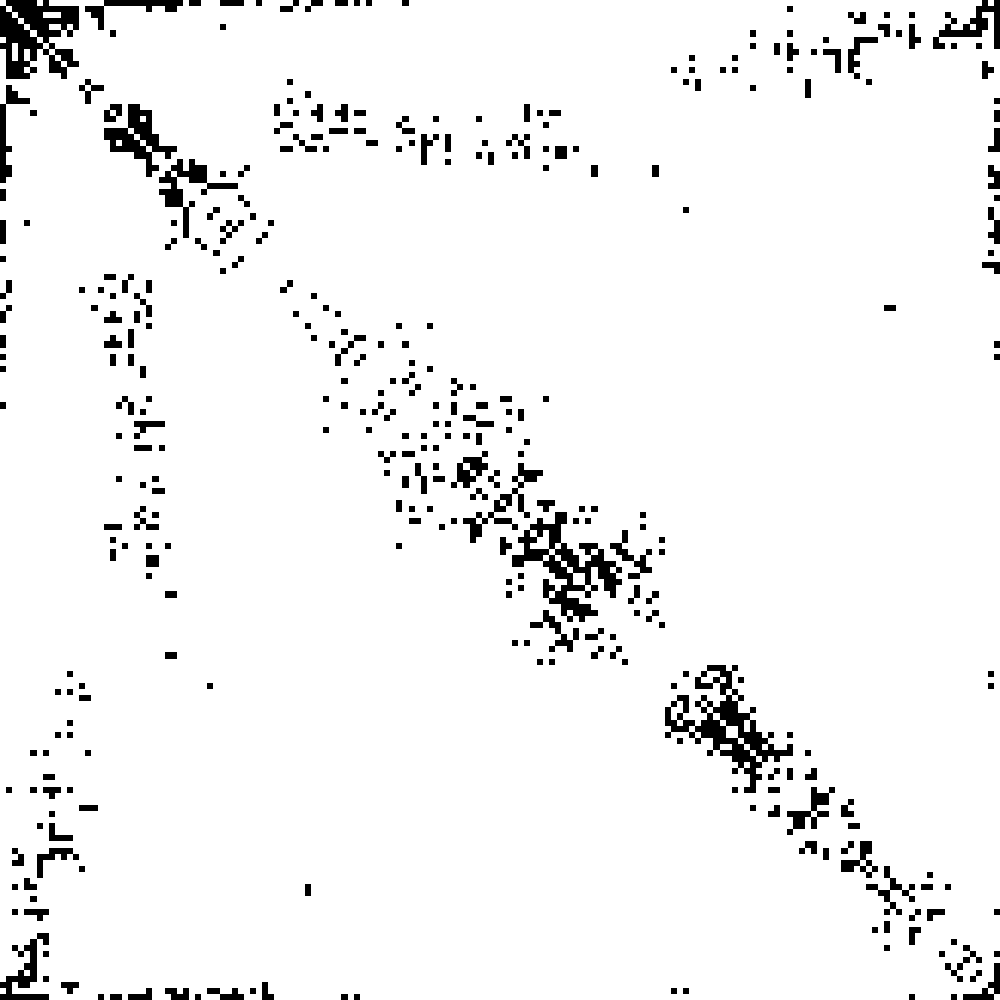
\includegraphics[width= 0.4\textwidth]{sorted_subject_matrix}%
    \hfill
    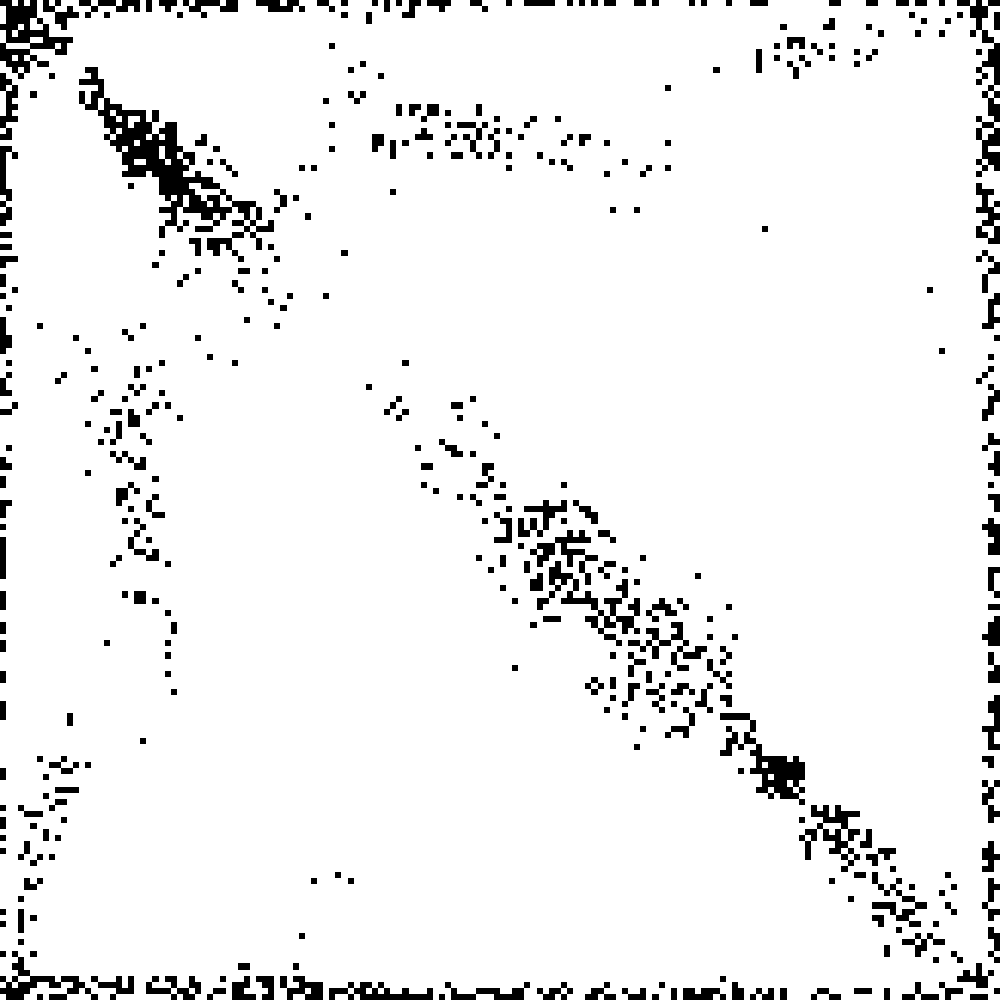
\includegraphics[width= 0.4\textwidth]{sorted_sample}%
    \caption{On the left, the ordered adjacency matrix of the original structural connectivity map, on the right the adjacency matrix of a sample of the graphon function MAP estimate.}
    \label{sortedadjacencymatrix}
\end{figure}

In figure \ref{sortedadjacencymatrix} homophily is visible, although other patterns are visible as well, such as a frame around the matrix. Similarly, the graphons that have been visualised until now all seem to curve up at the edge of the defined space, which seems to be an artefact of the estimation procedure.

\begin{figure}[H]
    \center
    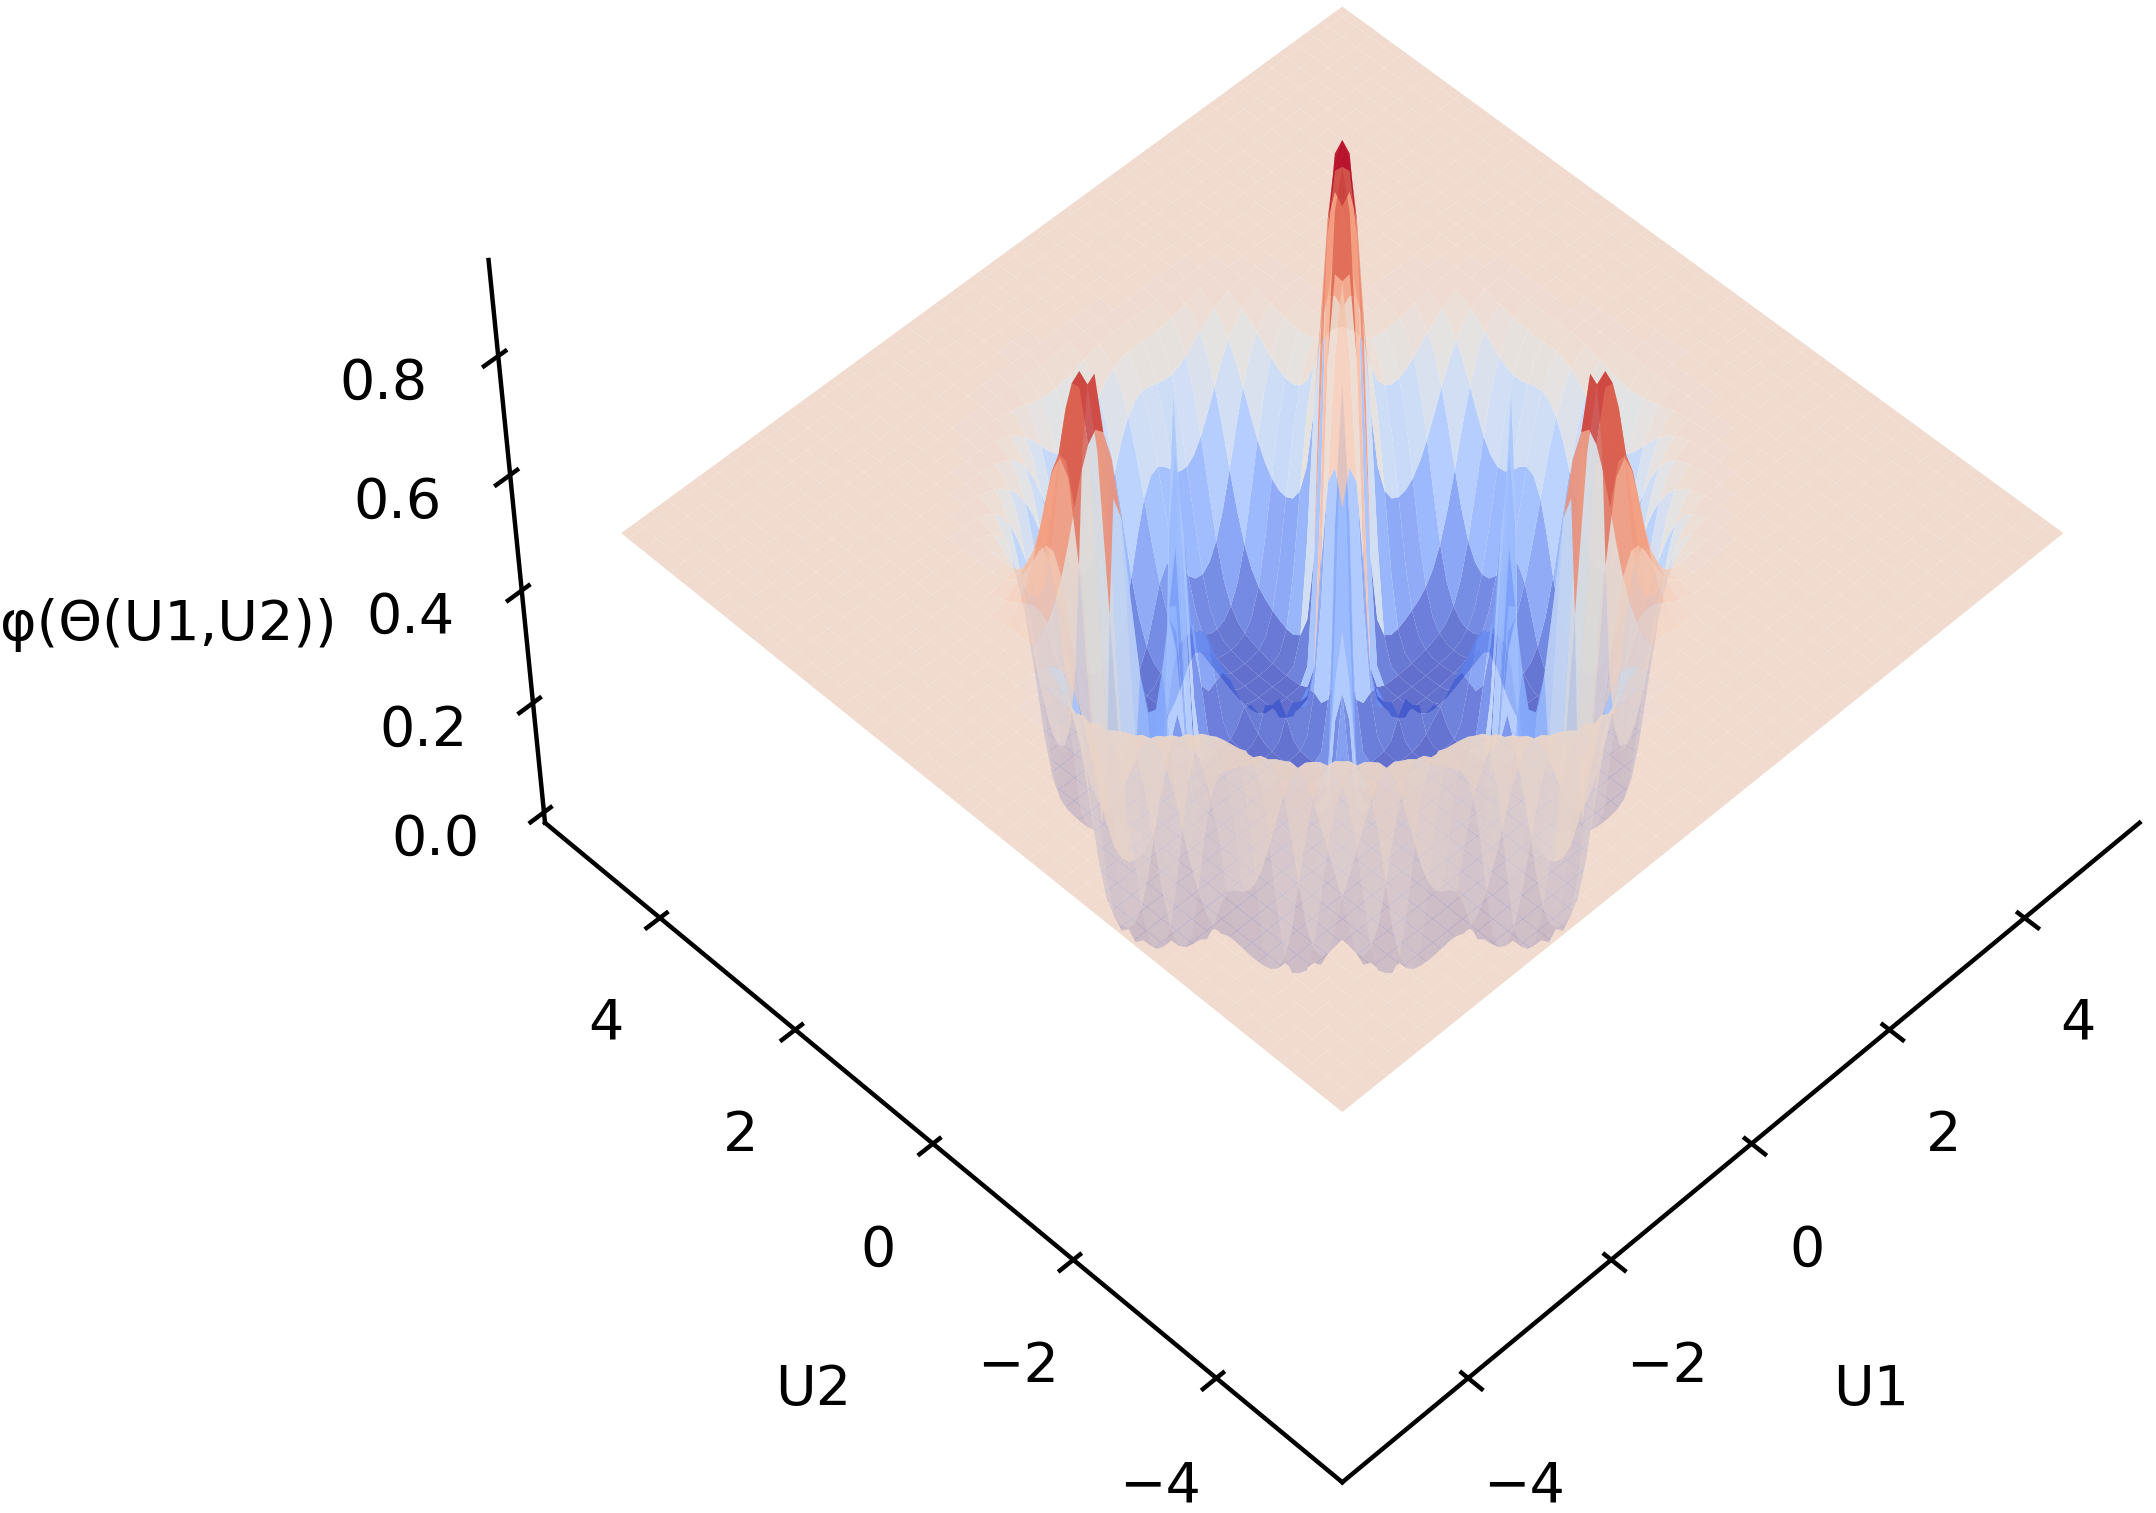
\includegraphics[width= 0.7\textwidth]{fakegraphon}%
    \caption{The same graphon as in \ref{visualisation 1} visualised with greater bounds.}
    \label{fakegraphon}
\end{figure}
\noindent
The graphon visualisation in figure \ref{fakegraphon} reveals why estimated graphons seem to curve up as they get to the edge. The further from the latent input points the graphon function is evaluated, the less is known about the value of the function there and the function goes to a neutral value of $0.5$.
% -------------------------------------------------------------------------------------------------------------------------------------------------------------------------------------------------------------------
 \chapter{Discussion}
\section{ Does graphon estimation improve upon other models link prediction abilities?}
The research question of this work can be answered in the positive, as the grapon beat out the contending models on average. However, the performance of all models was extremely homogeneous between graphs, which might indicate, that the graph data was very similar. This in turn might be a result of the consistency based thresholding that was applied to the dataset. In this procedure, edges that are less consistent across the dataset are removed first during thresholding, which contributes to inter subject similarity. It is surprising however, that the graphs of the subjects were highly homogeneous even at a graph density of 20 percent. Nevertheless, the strong link prediction capability of the RFM could be demonstrated, which answers the research question and affirms the first hypothesis.
\section{Comparing Graphons}
The second hypothesis of this paper revolved around the idea that Graphons can serve as a medium to compare graphs in. However, taking a sampling approach as was done in this experiment is not sufficient to detect small differences in graph structure. Even if the graphon model learns a graphon perfectly, sampling from said graphon would introduce randomness again, meaning that most likely only large differences can be seen in the graphon samples. This procedure is thus inappropriate for a dataset such as MICA-MICs, which is highly homogeneous. There has been some work on translating graph properties into the space of graphons by \citeA{Medina2020}, but their approach requires integrating over the graphon function, which is not trivial with a Gaussian Process approximation of the graphon function. This does seem like an opportunity to make the graphon relevant for connectomics, as it cannot be used as an intermediary for graph comparison using the RFM at this moment.
\section{Graphon Similarity Healthy Adults}
Given the aforementioned limitations of the graphon model, it is not possible to give a well defined answer to the question of whether the graphons of healthy adults are similar. According to the graph measures that describe the MICA-MICs data, the networks are already highly similar, whereas samples from graphon estimates have higher variance in the same graph measures. This indicates that at this point, the graphon model is not the right tool to discuss subject similarity.
\section{Modelling Performance}
The samples drawn from graphons trained on have high variance compared to the observed brain networks. This implies either that the model did not learn the relevant information, or that it is not possible to infer the model performance via the samples drawn from the graphon. However, the training on simulated data during the first experiment worked well, but in there the graph metrics were defined on samples in both cases, there the graphon model seems to have been successful, when comparing the graph measures.\\\\
Looking further into the first experiment, they do demonstrate that the RFM can learn networks with structures that are relevant to connectomics, such as networks exhibiting stochastic equivalence and Homophily.
\section{Stochastic equivalence}
Graphon estimation models are in general capable of learning stochastic equivalence, that is to say that they can model the situation that nodes i and j have the same probability of being linked with other nodes from the same group. 
This was shown in experiment \ref{provengraphonexperiment}, as the community graphon in that experiment exhibited stochastic equivalence which can be seen in figure \ref{estimatedcommunitygraphon}. 
Given that experiment \ref{provengraphonexperiment} showed the ability of the model to learn stochastic equivalence, it is interesting that the graphons visualised throughout the experiment section, did not look similar to the community graphon. This might indicate that the networks that were analysed do not exhibit stochastic equivalence, or that the model failed to pick up on it.

\subsection{Homophily}
The graph attribute homophily describes how edges between similar nodes are more likely to exist than between dissimilar nodes. In the RFM we learn a latent position for the nodes of the network in a euclidean latent space, which suggests that similar nodes will be close together. We thus expect that a network exhibiting global homophily should reveal this trait by having connections appear along the diagonal of the adjacency matrix sorted on the latent MAP positions of the nodes. Again, in figure \ref{sortedadjacencymatrix} we can clearly observe this property, much stronger than any stochastic equivalence attribute. This suggests that either the structural connectivity network that we analysed shows more homophily than stochastic equivalence, or that the model failed to pick up on stochastic equivalence. But given that the RFM could learn the community graphon, it seems to be the case that the networks analysed exhibited little stochastic equivalence.
\section{Limitations of the RFM}
\subsection{Empty or Dense Sequences}
There is a debate within graphon modelling about whether graphon models and consequently random graph models are inherently misspecified for real networks. The theoretical definition of the graphon comes from the limit object of sequences of dense graphs \cite{lovasz2006}. This implies, that edge density of the graphs in such a sequence grows at least as $O(n^2)$, where $n$ is the size of the graph. This in turn is problematic, as many real world networks are sparse. This is also mentioned by the authors of the RFM, which state that they are aware of this situation and they see it as a model misspecification, but they do not address the issue further in terms of changes to the RFM \cite{lloyd2012}. \citeA{wolfe2013} on the other hand add a model parameter $p_n$ that directly determines the average density of the graphon, which is interesting, as they point out that this practice comes from stochastic block models.
Whereas the RFM assumes the graphon function to be unbounded, hence requiring a link function $\phi$ that squashes the value of $\Theta$ into the range $[0,1]$, the model by \citeA{wolfe2013} calculate the probability of an edge existing as $p_n*\Theta(\xi_{ij},\xi_{gh})$. $p_n$ is a value between $0$ and $1$ which depends on $n$ the size of the graph that is being sampled. As a consequence, this model can in theory model any kind of graph sequence, such as one that produces progressively sparse graphs as the size of the graph increases, but since the model is usually trained on a single observed graph, the value of $p_n$ might not be well defined for all $n$, as the authors remark.
It is furthermore unclear how this modification of the graphon model fits into the more general graphon theory, as it's not easy to see whether there are any further consequences of this modelling choice.
Nevertheless, this modelling choice has been repeatedly used, most recently by \citeA{chandna2020}.
\citeA{borgs2017} have mentioned, that recent papers have examined the applicability of graphons to sparse graphs, which concluded that graphon estimation models should also work for sparse graphs. While finally, \citeA{turnbull2020} mentioned that a reformulation of the graphon as edge exchangeable instead of vertex exchangeable graphs solves the density problem as well. There is no clear path forward yet, as multiple solutions have been proposed, while the extent of the problem has not been sufficiently researched. In the sampling experiment in section \ref{connectomesamplequaliyresults}, it was demonstrated that the sampled networks deviate from the observed network on average. The graph density of sampled graphs is on average lower than that of the original graph. It might be possible to improve upon the RFM by introducing an explicit density regulating variable as done by \citeA{chandna2020}, as this would make the density estimation an explicit part of the model, instead of an implicit part.
\subsection{Destructive Preprocessing}
A significant limitation of the current implementation of the model is the fact that it can only process binary graphs instead of weighted graphs or even real valued arrays. In connectomics and especially in structural connectomics, there is a debate going on with regards to the preprocessing steps that are performed before using graph theoretical models on the data. This has historically been done since graph theoretical measures were often only available for sparse binary graphs, or at least thought to be only applicable to these kinds of graphs. Recent research has shown however, that many graph theoretical measures are not negatively influenced by dense graphs \cite{civier2019}. Furthermore, \citeA{yeh2020} argued that setting arbitrary thresholds to prune spurious connections leaves the data no less biased than not pruning the data. Furthermore, pruning adds another step that hinders comparability between studies, as different studies choose different thresholds. In light of this development, it would be advantageous if the RFM could accommodate dense weighted graphs. This would certainly be feasible to do under a slightly different model definition. It would be interesting to see what the effects of this on the modelling results would be.
\subsection{Network Size}
A final drawback of the current implementation of the RFM using MCMC to draw samples from the posterior is that it scales at least with $O(n^3)$. Even though the subset of regressors approximation technique is employed, the runtime of the algorithm is very slow for networks with sizes above 100 nodes. This might be alleviated using a variational approach to approximating the posterior of the model. It would furthermore be interesting how such a model compares to an MCMC based model. 
% \subsection{MCMC Mixing}
% The MCMC technique is working for the model as it produces a realistic maximum a posteriori sample after a run of 2000 iterations. However, upon inspection of the graphs of individual traces of some variables, very little mixing can be observed. The posterior probability density does converge however, which is assumed to be sufficient grounds for determining the length of the sampling chain.
% -------------------------------------------------------------------------------------------------------------------------------------------------------------------------------------------------------------------
\chapter{Conclusion}\label{conclusions}
The graphon model offers some improvements above the stochastic block model in terms of link prediction. Furthermore, the graphon can learn graphons that are typically assumed to be relevant for networks in connectomics such as scale free graphons and community graphons. The RFM does not seem to struggle to learn either stochastic equivalence or homophily. However, this work has shown that the RFM does seem to struggle with finding a unique graphon for connectomics datasets, but this observation is only based on visual inspection and sampling quality, which might not be a fair assessment. This highlights that there are both challenges and opportunities relating to the graphon model. One of these is certainly extending the current implementation to work with real valued arrays instead of solely binary relations. Another is to translate graph properties to the space of graphons for better interpretability of the graphon. However, in their current state, Graphons are of limited use to the field of connectomics, as they seem to replace one complex object with another complex object. They do work well for link prediction, but as of right now, given their definition via the graphon function, they remain opaque to the practitioner. \\\\

The above challenges and feats of the model make it a promising technique in connectomics. As seen in the related work, the interpretability and flexibility of the graphon estimation approach, especially the Bayesian nonparametric formulation is already useful in understanding structural connectivity in multiple settings. However, the present work has shown that graphon estimation does suffer from problems, that need to be addressed in future research.

\appendix 
\chapter{Additional test}
\section{Density Reduction Test}
\begin{table}[h]
\caption{Area under the receiver operator characteristic (AUROC) values for the RFM model on the HCP dataset.}
\begin{tabular}{|l|l|}
\hline
 \textbf{Graph Density} & \textbf{AUROC} \\ \hline
 0.7 &  0.90   \\ \hline
  0.6 & 0.89  \\ \hline
 0.5 & 0.88  \\ \hline
 0.4 & 0.88 \\ \hline
 0.3 &  0.89  \\ \hline
 0.2 & 0.86  \\ \hline
 0.1 & 0.90  \\ \hline
 0.05 & 0.88  \\ \hline
 0.02 & 0.79  \\ \hline
 0.01 & 0.67  \\ \hline
\end{tabular}
\end{table}
\noindent
The above test was run to determine the network density that works best on the RFM. However, given that the network predictive ability stays roughly at 88 to 90 percent beyond 10 percent density, any of these densities work well. 20 percent density was chosen, as it allowed for more inter-subject variability in the data, given that consistency thresholding was applied to the data.
\section{Convergence}
Convergence was shown using trace plots of the unnormalised posterior density of the RFM model.
\begin{figure}[H]
    \center
    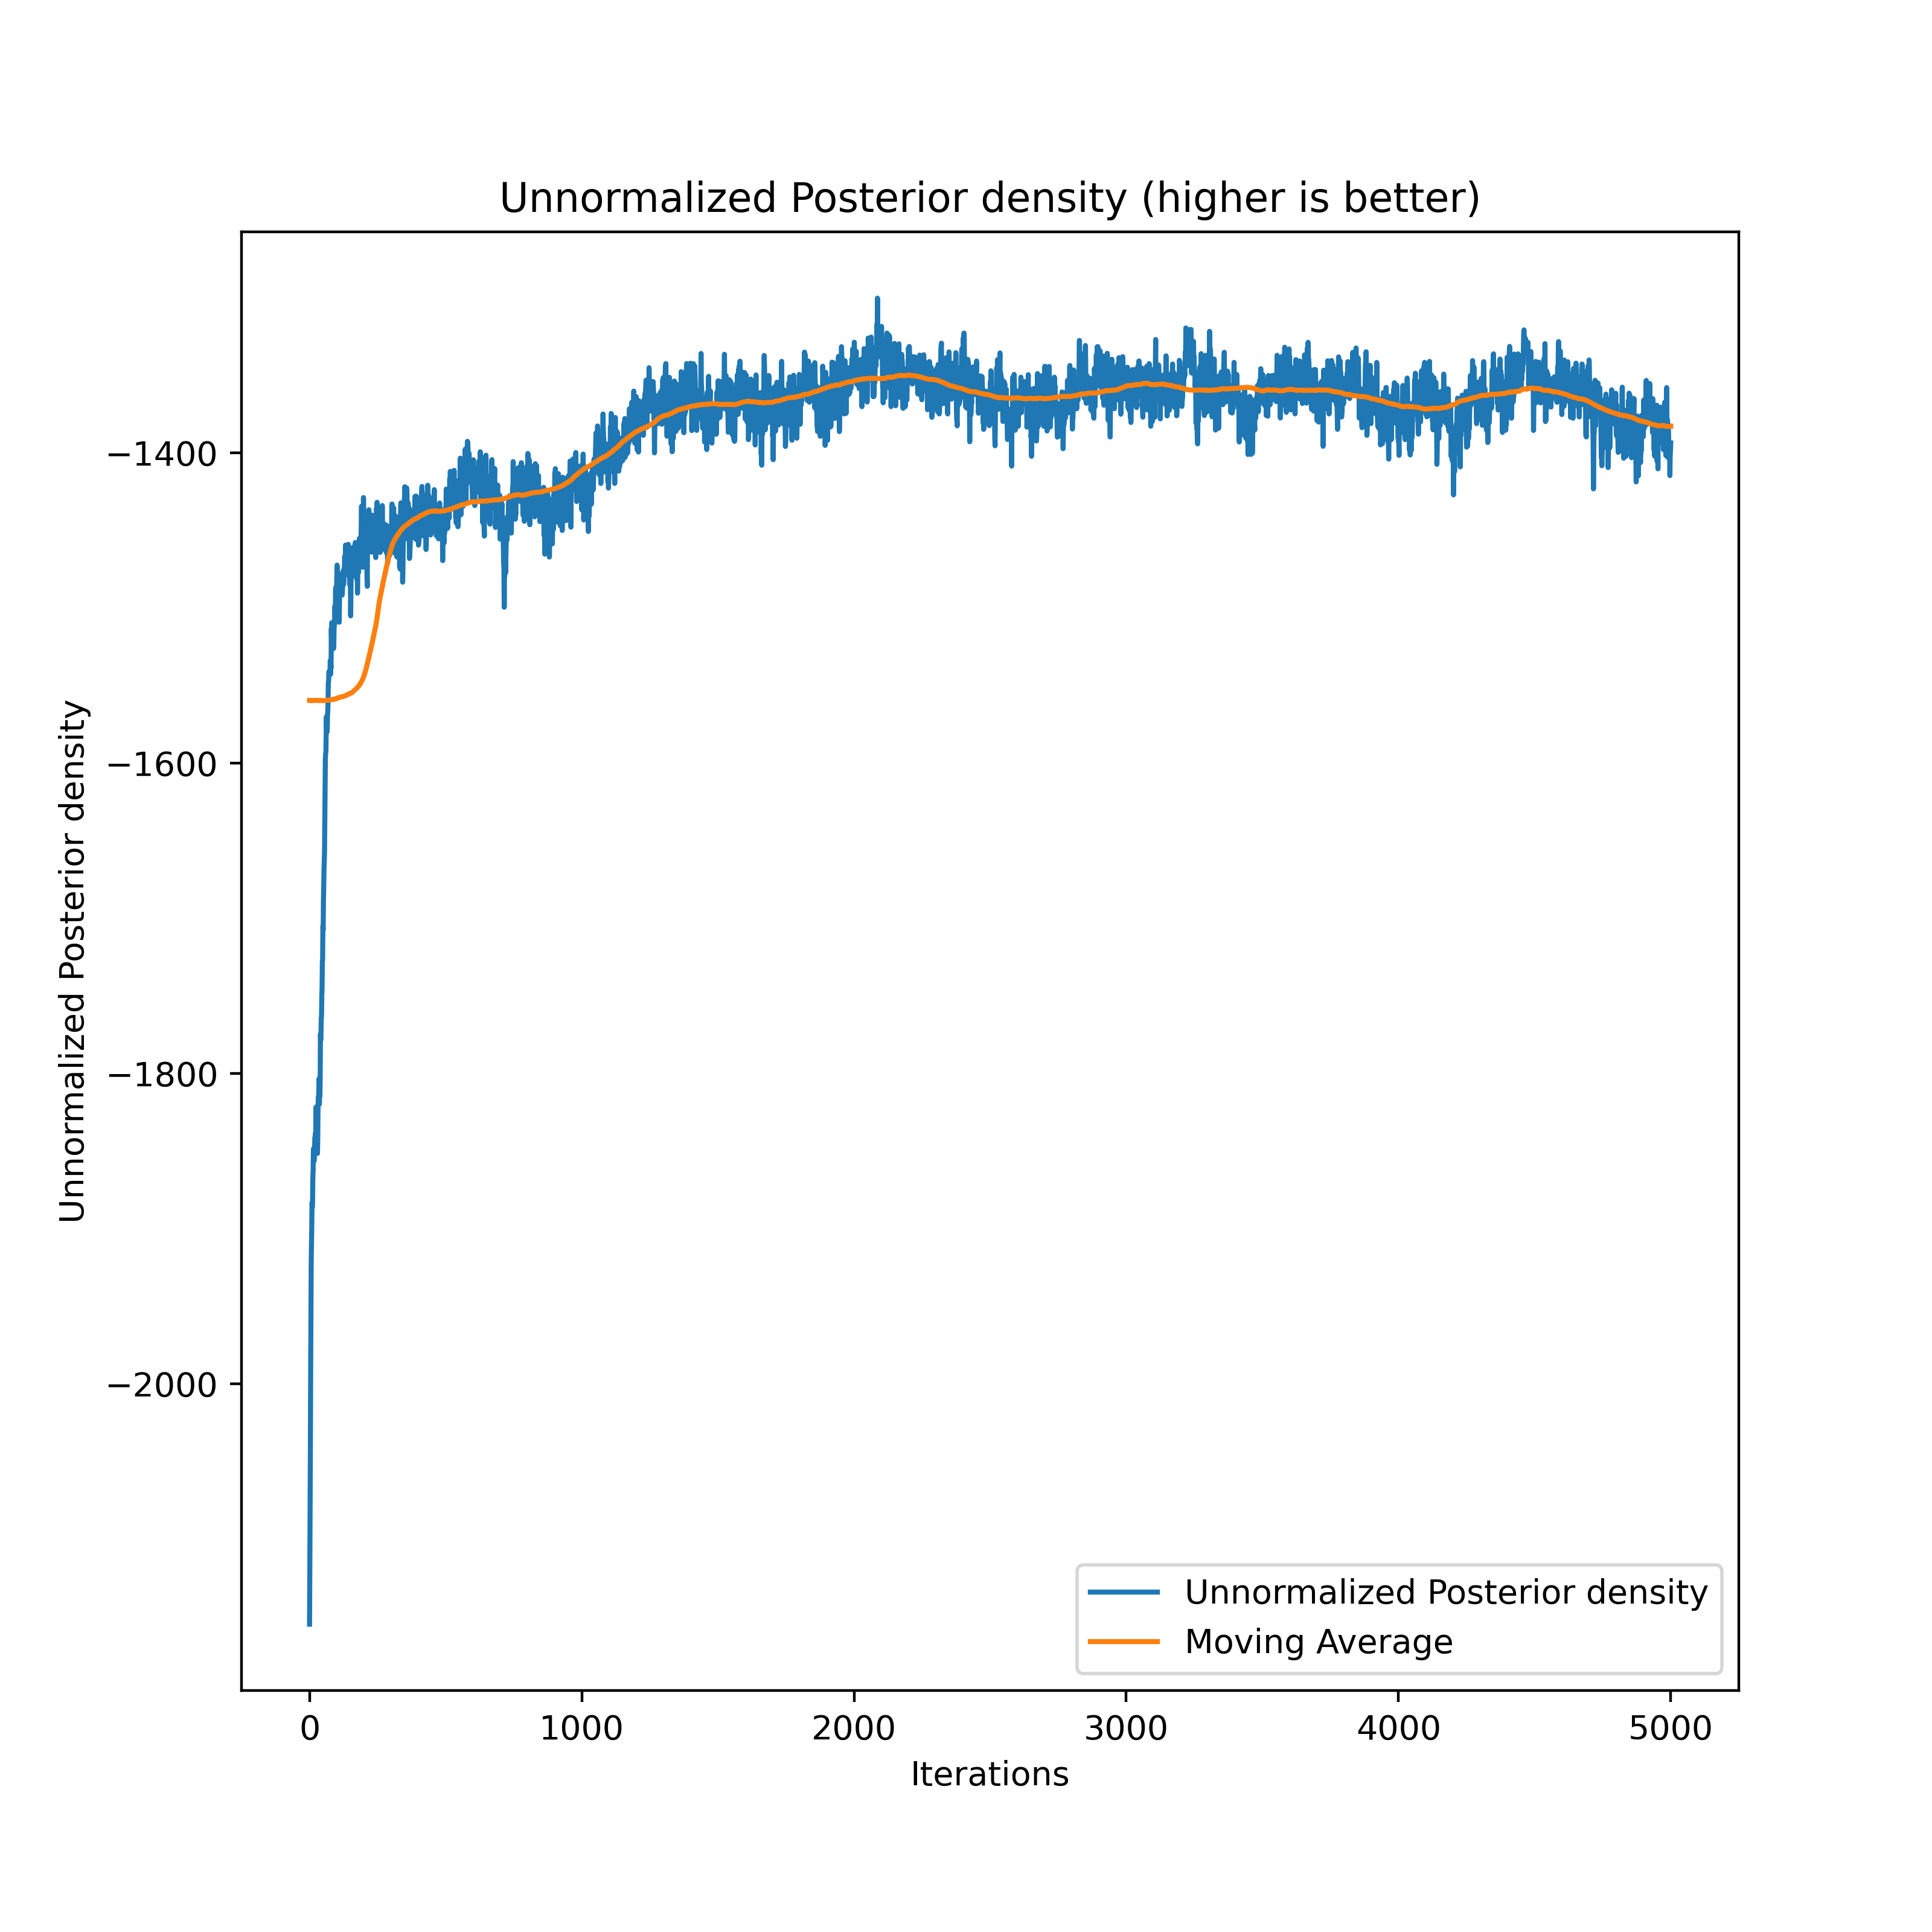
\includegraphics[width= 0.6\textwidth]{unnormalizedposteriordensity}%
    \caption{The RFM MCMC chain convergence was judged using the this traceplot of the unnormalised posterior density.}
\end{figure}

\nocite{funke2019}
\bibliography{bibliography}
\end{document}
% \mathcal{N}(0,I_n)